\documentclass[12pt, a4paper]{article}
\usepackage[margin=0.5in]{geometry}

\usepackage{color}
\usepackage[dvipsnames]{xcolor}
\usepackage{hyperref}
\hypersetup{
    colorlinks=true,
    linkcolor=blue,
    urlcolor=blue,
    linktoc=all
}

\usepackage{lipsum}

\usepackage{amsmath}
\usepackage{mathtools}
\usepackage{amssymb}
\usepackage{cancel}
\usepackage{bm}
\usepackage{dsfont}

\usepackage{booktabs,siunitx}

\usepackage{graphicx}
\graphicspath{ {./Graphics/} }
\usepackage{wrapfig}
% \usepackage[font=scriptsize]{caption}
\usepackage[font=small]{caption}
\setlength{\abovecaptionskip}{5pt plus 1pt minus 1pt} % Chosen fairly arbitrarily
% \captionsetup[figure]{font=small}

\usepackage{graphics}
\usepackage{xfrac}
\usepackage{array}
\setcounter{MaxMatrixCols}{40}

\usepackage{ulem} %just so I can strike through using \sout{text to be struck through}
  %also available:  \xout{text to be crossed out} for short diagonal lines crossing out each letter

\usepackage{enumerate}
\usepackage{enumitem}
\usepackage{multirow}

%inclusions carried over from past class homework formats
\usepackage{units}
\usepackage{fullpage}
\usepackage{alltt}
\usepackage{mathrsfs}
\usepackage{xcolor}
\usepackage{soul}

\usepackage{pgfplots}

\DeclarePairedDelimiter{\abs}{\lvert}{\rvert}
\newcommand*{\fontCourier}{\fontfamily{pcr}\selectfont}
\newcommand*\mean[1]{\overline{#1}}
\newcommand\scalemath[2]{\scalebox{#1}{\mbox{\ensuremath{\displaystyle #2}}}}

\setcounter{tocdepth}{5}
\setcounter{secnumdepth}{5}
% \setlength\parindent{0pt}

\usepackage{pdfpages}
\usepackage{Sweave}
\begin{document}
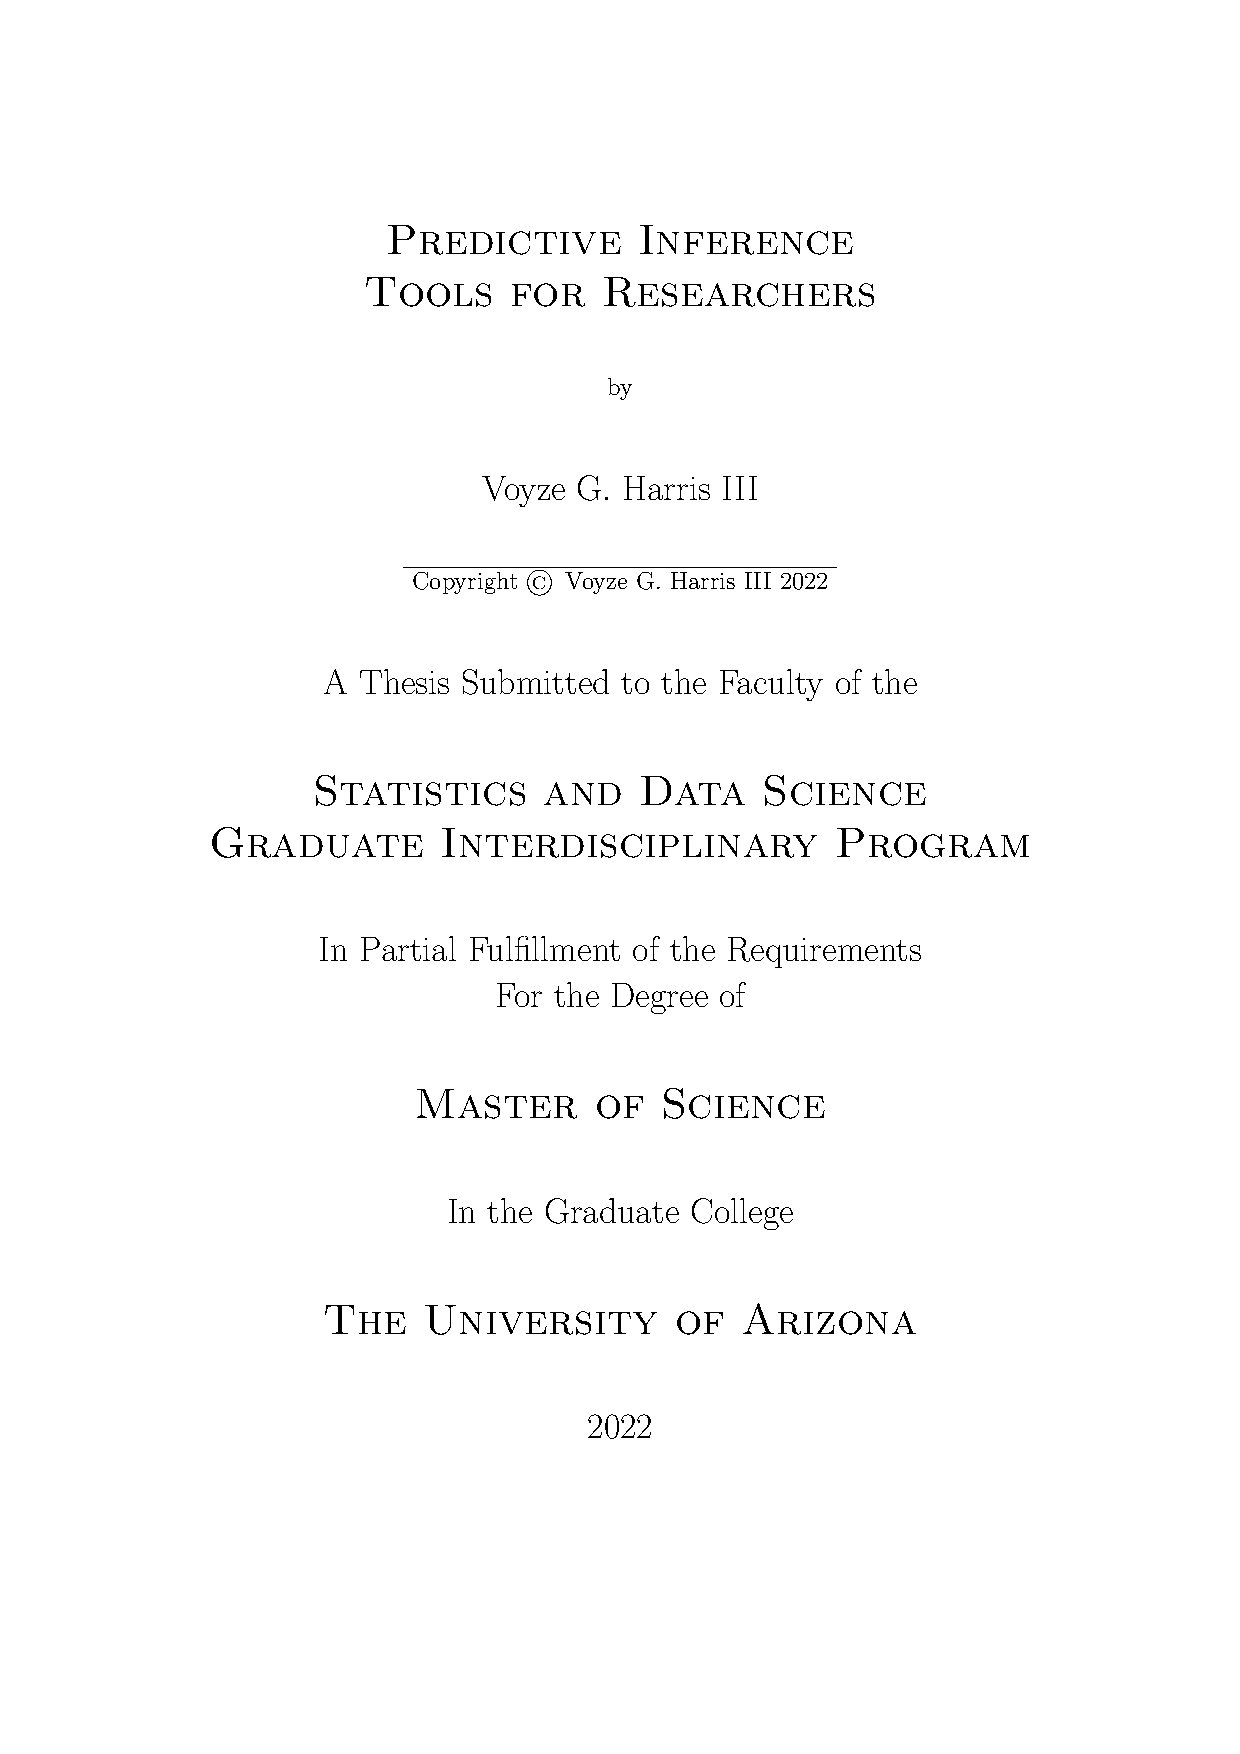
\includepdf{TitlePage_MastersThesis}

\includepdf{ThesisApprovalPage}
\Sconcordance{concordance:Thesis_v4.tex:Thesis_v4.Rnw:%
1 64 1 1 0 7 1 1 4 78 1 1 78 1 3 178 1 1 38 1 20 88 1 1 44 1 5 140 1 1 %
47 1 2 143 1 1 114 1 4 82 1 1 36 1 3 8 1 1 32 1 2 88 1 1 36 1 3 10 1 1 %
2 15 1 1 25 21 1 1 59 1 12 74 1 1 12 1 2 30 1 1 31 1 2 29 1 1 22 139 1 %
1 51 19 1 1 103 1 7 10 1}


\tableofcontents
\newpage


%%%%%%%%%%%%%%%%%%%%%%%%%%%%%%%%%
%%INTRODUCTION
%%%%%%%%%%%%%%%%%%%%%%%%%%%%%%%%%
\section{Thesis Abstract}
%% dean - I think you should include a bit more on predictive inferenc in the
%% abstract - add 2-3 sentences about how it's different from parametric
%% inference and why it's useful. You don't really need to much detail about the
%% function naming convention

An obstacle to widespread employment of Bayesian predictive inference in scientific research is the lack of suitable computing tools.  In this thesis I document several established useful models, and provide an applicable set of tools for statisticians.  For each of the included models, some basic notes on mathematical derivation are presented, and predictive inference is illustrated with examples.  For the details of the models and some of the examples I relied primarily on Seymour Geisser's \underline{Predictive Inference:  An Introduction} (1993) and Peter D. Hoff's \underline{A First Course in Bayesian Statistical Methods} (2009).\\

\noindent An R package has been developed, the main purpose of which is to provide the researcher with a means of producing random samples from predictive distributions.  For all the models, the package includes random sample generators.  For those models with analytical solutions, density and distribution functions are also provided.  The standard R naming convention for these function classes has been adopted:  density functions are prefixed with the letter ``d," distribution functions with the letter ``p," and random generation functions with the letter ``r."  Also included in all function names is the abbreviation ``pred" (for predictive) and an initialism or abbreviation identifying the model itself.  For example, the density function for the Beta-Binomial model is named ``\texttt{dpredBB()}."  The R code for each function is included in Appendix \textcolor{red}{X-insert link to appendix here}.



% \clearpage

\section{Introduction:  Predictive Inference}

My understanding of Bayesian Predictive Inference began with the University of Arizona course ``Bayesian Statistical Theory and Applications" under Dr. Edward Bedrick.  Since then it has been shaped by exposure to various sources, including articles by Bedrick and Dr. Dean Billheimer, and to a greater extent the aforementioned texts by Hoff and Geisser, and others, including \underline{Bayesian Data Analysis} by Andrew Gelman et. al., \underline{Statistical Prediction Analysis} by J. Aitchison and I.R. Dunsmore, and excerpts from \underline{The Signal and the Noise} by Nate Silver.  In the next section and what follows, the ideas expressed are an amalgam of what was learned from this body of scholarship.

  \subsection{Why Predictive Inference?}


I find persuasive the assertion that the main purpose of statistics is to predict future events based on observed data, and moreover that a statistical model may be judged chiefly by the quality of its predictions.  Predictions about meaningful quantities that are relevant to the object of study facilitate scientific progress in multiple ways.  Nate Silver notes:

\begin{quote}
Prediction is important because it connects subjective and objective reality. Karl Popper, the philosopher of science, recognized this view. For Popper, a hypothesis was not scientific unless it was falsifiable—meaning that it could be tested in the real world by means of a prediction.
\end{quote}

\noindent Billheimer emphasizes the improvement of scientific accuracy and reproducibility Bayesian prediction provides by ``shifting our focus from `finding differences' among hypothetical parameters to predicting observable events based on our current scientific understanding."  Focus on observed data enables corroboration or refutation of current hypotheses through future experimentation, and informs decision-making by summarizing quantities of direct interest to the researcher.  Bayesian predictive inference shifts the focus of statistical analysis from estimation of hypothetical parameters to statements about concrete observables.\\

\noindent It is not the intent of this thesis to suggest that parametric inference should be abandoned in statistical analyses.  Conventional statistical inference techniques are useful for summarizing information about large quantities of data in a small number of usable values (parameter estimates), and leveraging such summaries to determine whether a particular problem merits continued attention. Indeed, the scientific discipline of mathematical statistics has developed along parametric lines, imparting greater efficiency to the solving of idealized versions of problems. However, this focus on parameters has largely ignored the impact of observable quantities which may exhibit distributions very different from our (idealized) standard models. In support of prediction in general, and Bayesian prediction in particular, I return to Nate Silver:\\

\begin{quote}
Making predictions based on our beliefs is the best (and perhaps even the only) way to test ourselves. If objectivity is the concern for a greater truth beyond our personal circumstances, and prediction is the best way to examine how closely aligned our personal perceptions are with that greater truth, the most objective among us are those who make the most accurate predictions. Fisher’s statistical method, which saw objectivity as residing within the confines of a laboratory experiment, is less suitable to this task than Bayesian reasoning.
\end{quote}



\noindent Prediction is a means of discriminating between scientific hypotheses. Generally, a model may be judged by the quality of its predictions.  Given competing models, the better predictor will be given more weight, and a useful model increases in utility as its predictive capability improves.  With Bayesian inference, prior informed opinion about parameter distributions, updated with knowledge gained through observations, yields better predictions with each update.\\


\begin{wrapfigure}{R}{0.30\textwidth}
  \begin{center}
    
\includegraphics[width=0.28\textwidth]{./Graphics/PassThePigs/PtPBox}
  \end{center}
  \caption{Pass The Pigs\textsuperscript{\circledR}}
\end{wrapfigure}

\noindent To illustrate the potential difference between Bayesian prediction and the use of plug-in estimators, consider the game Pass the Pigs\textsuperscript{\circledR}, a push-your-luck dice game in which the ``dice" are actually rubber pig figures.  Two pig dice are thrown, and points are scored according to the combination of positions in which they come to rest.  Details about the game can be found on Wikipedia here: \url{https://en.wikipedia.org/wiki/Pass_the_Pigs}\\

%% DONE how about a picture of a pig in razorback position?  e.g. via cell phone?

\begin{wrapfigure}{L}{0.30\textwidth}
  \begin{center}
    
\includegraphics[width=0.28\textwidth]{./Graphics/PassThePigs/Razorback}
  \end{center}
  \caption{Razorback}
\end{wrapfigure}

\noindent For the purpose of this example, consider the probability of a single pig landing in the ``Razorback" position, which occurs when the pig is lying on its back with its legs extended upward.  The irregular shape of the pig makes it difficult to assign probabilities to results other than by means of experimentation.  Such an experiment was conducted at Duquesne University, and an article describing the experiment as well as Bayesian predictive inference performed on the results appeared in the \textit{Journal of Statistics Education} Volume 14, Number 3, in 2006.  The article can be accessed here:  \url{http://jse.amstat.org/v14n3/datasets.kern.html}. Of the $11,954$ recorded results for individual pigs, approximately $22.4\%$ were Razorbacks.\\

\noindent Suppose in new data $t=4$ Razorbacks have been observed out of $N=10$ tosses of a single pig die, suggesting a straightforward binomial distribution with $\theta =$ Pr(Razorback) $= t/N = 0.4$. Taking the Duquesne experiment into consideration, we'll perform Bayesian prediction using various Beta prior distributions for $\theta$: $\theta\sim\text{Beta}(2,8)$, $\theta\sim\text{Beta}(22,78)$, and $\theta\sim\text{Beta}(224,776)$, and compare these results to predictions obtained from the plug-in estimator $\theta = 0.4$.   Any number of prior distributions on $\theta$ would satisfy the condition that $E(\theta) \approx 0.224$, suggested by the prior information.  The specific choice of a Beta prior is made largely for computational convenience.\\

\noindent The researcher wants to predict how many Razorbacks will result from some number $M$ of future pig die rolls.  In this example, $M=100$ was used.  The density curves in the plot below show the influence of the choice of prior parameters on the location and variance of the predictive distribution.  Essentially, each pair of shape parameters $(\alpha,\beta)$ in the Beta prior reflects the researcher's level of reliance on the results of the Duquesne experiment, with the ``weight" given to that knowledge increasing with the shape parameters by orders of magnitude.  The choice of parameters might be influenced by such things as pig tossing method (perhaps the researcher is throwing them by hand rather than dropping them by the carefully controlled method used in the Duquesne experiment), or by a need to account for pig-to-pig variation, or anything else the researcher believes introduces a deviation from the events upon which the prior information is based.  Use of the scaled-up Big Pigs\texttrademark variant, for example might give reason to use a very low-weighted prior such as $\theta\sim\text{Beta}(2,8)$.

\begin{figure}[ht]
  \centering
  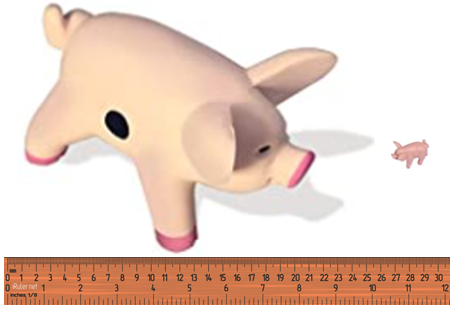
\includegraphics[width=0.9\textwidth]{./Graphics/PassThePigs/PigSize_wRuler}
  \caption{Big Pigs\texttrademark to Original (Approximate Scale)}
\end{figure}


\noindent The plot and table below illustrate the effects of the Bayesian prediction method. Perhaps most notable is the location disparity between the plug-in (Binomial) prediction and the family of Bayesian (Beta-binomial) predictive distributions.  The consideration of prior knowledge is also shown to have a significant effect.  In this example, the strong influence of the choice of shape parameters for the Beta prior on the mean and variance of the predictive distribution provides options for the future prognosticator. If a new set of trials closely duplicates the Duquesne experimental conditions, for example, predictions might be based on the result from the Beta$(224,776)$ prior.  A lower-weighted prior might be used for any experimental element the researcher believes introduces a deviation from the knowledge upon which the prior information is based.

\vspace{1cm}

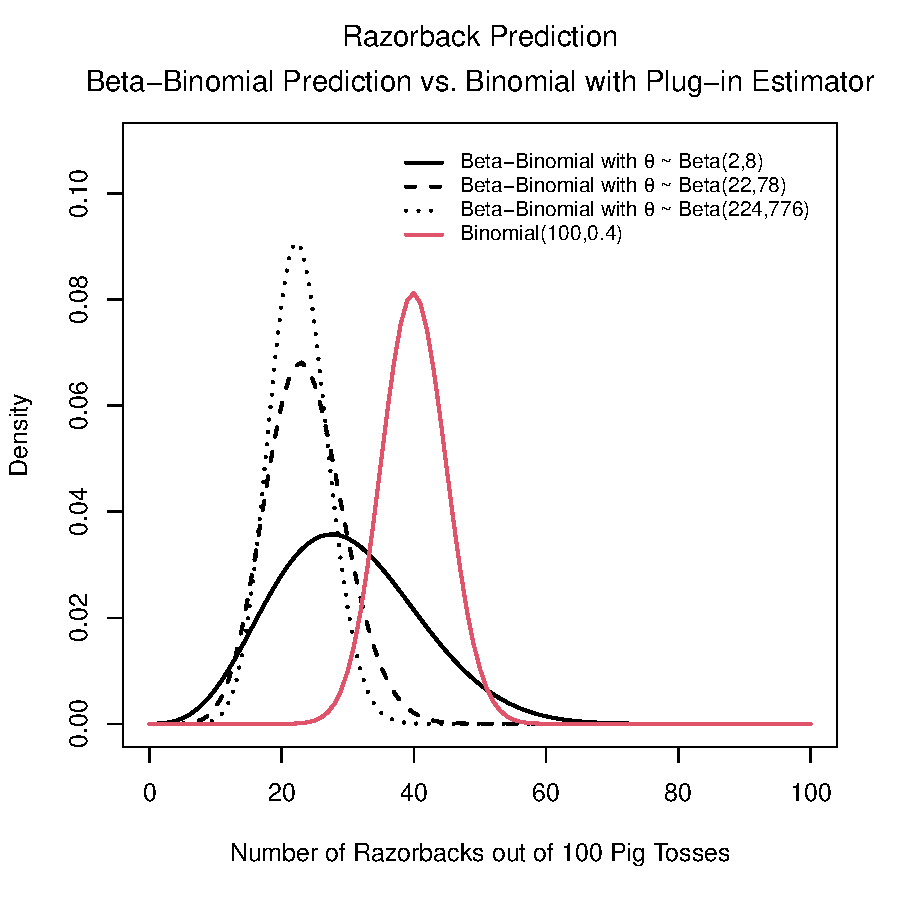
\includegraphics{Thesis_v4-002}

\vspace{1cm}

\begin{center}
  \begin{tabular}{l c c c c }
  \toprule
  \multicolumn{5}{c}{\large \#Razorbacks Predicted out of 100 Tosses}          \\
  \multicolumn{1}{c}{\textbf{Prediction Method}} & \multicolumn{1}{c}{$\textbf{(}\boldsymbol\alpha,\boldsymbol\beta\textbf{)}$}  & \multicolumn{1}{c}{\textbf{Prior Mean }$\textbf{E(}\boldsymbol\theta\textbf{)}$}  & \multicolumn{1}{c}{\textbf{Prediction Mean}} & \multicolumn{1}{c}{\textbf{SD}}\\
        \midrule
        Beta-Binomial & (2,8) & 0.2 & 29.3 & 10.75 \\
        \midrule
        Beta-Binomial & (22,78) & 0.22 & 23.48 & 5.74\\
        \midrule
        Beta-Binomial & (224,776) & 0.224 & 22.54 & 4.4 \\
        \midrule
        Binomial$(100,0.4)$ & -- & -- & 40 & 4.9 \\
  \bottomrule
  \end{tabular}
\end{center}

\vspace{1cm}

\noindent The differences in the results of the two prediction methods are easy to see in this case. Unlike the Bayesian approach, the binomial-only model uses only the observed data, does not account for any uncertainty in the binomial parameter ($\theta$), and ignores historical info about Razorback frequency.  If speculating whether the number of razorbacks out of the next 10 pig tosses will be greater than, say, 3, the indications of the two analysis approaches contradict each other.  The statistically savvy wagerer of course realizes that the 10 die throws informing the plug-in results do not guarantee high confidence.  A much less risky option for the bettor is the Bayesian method with a suitable prior parameterization.


\clearpage

  \subsection{The Bayesian Parametric Prediction Format}

\noindent We want to predict future outcomes based on current knowledge.
Specifically we're asking: for observed values $Y_1 = y_1,...,Y_n = y_n$, what
is likely to be the value of the next observation, $\tilde{Y}$?  We want to compute $Pr(\tilde{Y}|y_1,...,y_n)$, where $y_1,...,y_n$ are
conditionally independent and identically distributed (i.i.d.) with respect to  a population parameter (or parameters) $\theta$.  We assign prior distribution
 $\pi(\theta)$ based on some existing knowledge or beliefs.  Here we are careful to satisfy ourselves that $Y_1,...,Y_n$ are \textit{exchangeable}, which
 enables us to rely on de Finetti's representation theorem for the conditional independence assumption.  Exchangeability means essentially that the order of the observations conveys no information affecting the distribution of the data.  That is, $p(Y_1,...,Y_n) = p(Y_{\pi_1},...,Y_{\pi_n})$ for any permutation $\pi_1,...,\pi_n$ of the indices $1,...,n$.\\

\begin{quote}
  \textbf{De Finetti's Theorem:  } Let $Y_i\in\mathcal{Y}$ for all $i\in\{1,2,...\}$.  Suppose that, for any $n$, our belief model for $Y_1,...,Y_n$ is exchangeable. Then our model can be written as

  $$p(y_1,...,y_n) = \int\left\{\prod_1^n p(y_i|\theta)\right\}p(\theta)d\theta$$

  for some parameter $\theta$, some prior distribution on $\theta$ and some sampling model $p(y|\theta)$.  The prior and sampling model depend on the form of the belief model $p(y_1,...,y_n)$.\\
\end{quote}

\textcolor{blue}{How is the following paragraph?}

\noindent Simply put, exchangeability of data implies (conditional) independence and identical distribution (i.i.d.) with respect to a parameter with some prior distribution. The converse is immediate from the definition of marginal probability and the commutative property of multiplication. Hoff summarizes these ideas like this (p. 29):\\


\[
\begin{rcases}
Y_1,...,Y_n|\theta \text{ are i.i.d}\\
\theta\sim\pi(\theta)
\end{rcases} \Leftrightarrow Y_1,...,Y_n \text{ are exchangeable for all } n
\]

\vspace{5mm}

\noindent The derivations throughout this thesis assume exchangeability, so we can formulate predictive probability as follows:

\begin{flalign}
  p(\tilde{Y} = \tilde{y} | Y_1 = y_1,...,Y_n = y_n) &= \frac{p(\tilde{y},y_1,...,y_n)}{p(y_1,...,y_n)}\nonumber\\
  &\nonumber\\
  &=\frac{\int p(\tilde{y},y_1,...,y_n | \theta)\pi(\theta) d\theta}{p(y_1,...,y_n)}\nonumber\\
  &\nonumber\\
  &= \frac{\int p(\tilde{y}|\theta)p(y_1,...,y_n | \theta)\pi(\theta) d\theta}{p(y_1,...,y_n)}\nonumber\\
  &\nonumber\\
  &= \frac{\int p(\tilde{y}|\theta)p(\theta|y_1,...,y_n) p(y_1,...,y_n) d\theta}{p(y_1,...,y_n)}\nonumber\\
  &\nonumber\\
  &= \int p(\tilde{y}|\theta) p(\theta|y_1,...,y_n) d\theta \label{BayesianPredictiveFormat}
\end{flalign}

\noindent For prediction, we need only to characterize the observed data $(y_1,...,y_n)$, conditionally independent with respect to  $\theta$, and supply a suitable prior distribution $\pi(\theta)$.  Then we compute posterior $p(\theta|y) = p(y|\theta)\pi(\theta)/\int_\theta p(\theta)p(y|\theta)d\theta$ and generate a prediction using   (\ref{BayesianPredictiveFormat}).  In some cases the integral has an analytical solution, while in others we evaluate it through monte carlo (MC) sampling.



\clearpage

\section{Predictive Problems with Conjugate Priors}

\noindent When data can be modeled with a distribution that suggests a conjugate prior for the parameter(s) of interest, and those parameters can reasonably be represented by that conjugate prior, the posterior calculations are greatly simplified.  The four classes of models addressed in this section all exhibit this feature.  The first three are single-parameter exponential families and have closed-form solutions for prediction.  The fourth is a two-parameter exponential family with unkown mean and variance.  While this one does not admit an analytical solution, prediction is easily accomplished by means of simple monte carlo sampling.  The four classes of predictive models presented in this section are:
\begin{itemize}
  \item Beta-Binomial ($T = \sum Y\sim$ Binom$(N,\theta)$ with $\theta\sim$ Beta)
  \item Exponential-Gamma ($Y\sim$ Exp$(\theta)$ data with $\theta\sim$ Gamma)
  \item Poisson-Gamma ($Y\sim$ Poi$(\theta)$ data $\theta\sim$Gamma)
  \item Normal-Inverse Gamma ($Y\sim$ Normal$(\theta,\sigma)$ data with $\theta\sim$ Normal and $\sigma\sim$ Inverse Gamma)
\end{itemize}

\noindent Throughout this section, $N$ is used for the observed data sample
size, and $S$ is the size of the desired random sample of predictions. The predicted future result
is indicated by surmounting the variable name with a tilde.  For example, when the observed data is represented by $y$, the prediction is designated $\tilde{y}$. Parameter names are clearly indicated as they appear.

  \subsection{Prediction of Future Successes:  Beta-Binomial (Geisser p. 73)}


    \subsubsection{Derivation}

    \noindent Let $Y_1,...,Y_N$ be exchangeable binary variables, and therefore conditionally i.i.d.  with respect to some parameter $\theta$. That is, Pr$(Y_i = 1) = \theta$, with $Y_i = 1$ indicating success and $Y_i = 0$ indicating failure.  The number of observed successes can be represented by $T = \sum Y_i$, which is sufficient for $\theta$ and has a binomial$(N,\theta)$ distribution.  That is,

      $$Pr(T = t|\theta) = {N\choose t}\theta^t(1-\theta)^{N-t}.$$

      \vspace{5mm}

\noindent Assuming $\theta\sim\text{Beta}(\alpha,\boldsymbol\beta)$, we have prior distribution

      \vspace{5mm}

      $$\pi(\theta) = \frac{\Gamma(\alpha + \beta)\theta^{\alpha - 1}(1 - \theta)^{\beta - 1}}{\Gamma(\alpha)\Gamma(\beta)}.$$

      \vspace{5mm}

\noindent The posterior distribution of $\theta$ given $Y_1,...,Y_N$, then, is

      \vspace{5mm}


\begin{flalign*}
  p(\theta|Y_1,...,Y_N) = p(\theta|t) &= \frac{p(t|\theta)\pi(\theta)}{\int p(t|\theta)\pi(\theta)d\theta}\\
  &\\
  &= \frac{{N\choose t}\theta^t(1-\theta)^{N-t}\frac{\Gamma(\alpha + \beta)\theta^{\alpha - 1}(1 - \theta)^{\beta - 1}}{\Gamma(\alpha)\Gamma(\beta)}}{\int{N\choose t}\theta^t(1-\theta)^{N-t}\frac{\Gamma(\alpha + \beta)\theta^{\alpha - 1}(1 - \theta)^{\beta - 1}}{\Gamma(\alpha)\Gamma(\beta)}d\theta}\\
  &\\
  &= \frac{\theta^{t+\alpha-1}(1-\theta)^{N-t+\beta-1}}{\int \theta^{t+\alpha-1}(1-\theta)^{N-t+\beta-1}d\theta}\\
  &\\
  &= \frac{\Gamma(N+\alpha+\beta)}{\Gamma(t+\alpha)\Gamma(N-t+\beta)}\theta^{t+\alpha-1}(1-\theta)^{N-t+\beta-1}\\
  &\\
  &= \text{Beta}(t+\alpha,N-t+\beta)
\end{flalign*}

\noindent Note that the ratio of Gamma functions in the final step appears as a scaling constant that enables the Beta$(t+\alpha,N-t+\beta)$ density function under the integrand in the denominator of the previous step to resolve to 1.

      \vspace{5mm}

      \noindent We want to predict the number $\tilde{T}$ of successes in a future experiment involving $M$ binary observations.  That is, $\tilde{T} = \sum_{i=1}^M Y_{N+i}$, and we have Beta-Binomial predictive distribution

\begin{flalign}
  \text{Pr}[\tilde{T} = \tilde{t}|T=t]
  &= \int p(\tilde{T} = \tilde{t}|\theta)p(\theta|t)d\theta\nonumber\\
  &\nonumber\\
  &= \int {M\choose \tilde{t}}\theta^{\tilde{t}}(1-\theta)^{M-\tilde{t}}\frac{\Gamma(N+\alpha+\beta)}{\Gamma(t+\alpha)\Gamma(N-t+\beta)}\theta^{t+\alpha-1}(1-\theta)^{N-t+\beta-1}d\theta\nonumber\\
  &\nonumber\\
  &= \frac{M!}{\tilde{t}!(M-\tilde{t})!}\frac{\Gamma(N+\alpha+\beta)}{\Gamma(t+\alpha)\Gamma(N-t+\beta)}\int\theta^{\tilde{t}+t+\alpha-1}(1-\theta)^{M+N-\tilde{t}-t+\beta-1}d\theta\nonumber  \\
  &\nonumber\\
  &= \frac{\Gamma(M+1)\Gamma(N+\alpha+\beta)\Gamma(\tilde{t}+t+\alpha)\Gamma(M+N-\tilde{t}-t+\beta)}{\Gamma(\tilde{t}+1)\Gamma(M-\tilde{t}+1)\Gamma(t+\alpha)\Gamma(N-t+\beta)\Gamma(M+N+\alpha+\beta)},\label{betaBinomial_pred}
\end{flalign}

\noindent an impressive combination of Gamma functions.  Note that the last two factors in the numerator together with the final factor in the denominator comprise the reciprocal of the scale factor corresponding with the Beta$(\tilde{t}+t+\alpha,M+N-\tilde{t}-t+\beta)$ kernel in the integrand, enabling the integral to resolve to 1.


% \clearpage

    \subsubsection{R Implementation (Beta-Binomial)}

This result has been used to create R functions \texttt{dpredBB()}, \texttt{ppredBB()}, and \texttt{rpredBB()} for the Beta-Binomial predictive distribtuion for density, cumulative probability, and random sampling, respectively (see appendix for the R code).  The density function \texttt{dpredBB()} relies on the R function \texttt{lgamma()} to evaluate the numerator and denominator of the predictive distribution (\ref{betaBinomial_pred}) factor by factor logarithmically, and then exponentiates for the final result, evaluated at the desired integer value (or vector of values) $\tilde{y}$ input by the user.  The cdf \texttt{ppredBB()} simply calls \texttt{dpredBB()} and returns the cumulative sum of that discrete set of results.  The random sampler \texttt{rpredBB()} makes use of the inverse transform method and the output from the cdf \texttt{ppredBB()}.  Calls to these functions appear as follows:

\begin{center}
  \texttt{dpredBB(tpred,N,t,M,a,b)}\\
  \texttt{ppredBB(tpred,N,t,M,a,b)}\\
  \texttt{rpredBB(S,N,t,M,a,b)}\\
\end{center}

\noindent where

\begin{flalign*}
  \texttt{tpred} &= \tilde{t} \text{, the number (or vector of numbers) of successes in a future experiment }\\
  &\text{ involving } M \text{ binary observations} \\
  \texttt{N} &= \text{the number of observations in the current data set}\\
  \texttt{t} &= \text{the number of successes out of the N observations in the current data set}\\
  \texttt{M} &= \text{the number of binary observations in a future experiment}\\
  \texttt{a} &= \alpha \text{, the first shape parameter of the Beta prior}\\
  \texttt{b} &= \beta \text{, the second shape parameter of the Beta prior}\\
  \texttt{S} &= \text{the desired random sample size; that is, the number of future experiments }\\
  &\text{ of size } M \text{ for which a predicted number of successes is desired}\\
\end{flalign*}

    \subsubsection{Example}

The functions \texttt{dpredBB()} and \texttt{rpredBB()} were used in the Pass The Pigs\textsuperscript{\circledR} example in the introduction.  Here, all three functions are exercised in an imagined experiment using the Big Pigs\texttrademark variant.  Suppose $t=7$ Razorbacks have been observed out of $n=10$ tosses of Big Pigs\texttrademark, and the researcher has settled on prior distribution Pr(Razorback) = $\theta\sim\text{Beta}(2,8)$.  For $M = 10$ future observations, how many successes are predicted?  The figures below show the predictive distribution from \texttt{dpredBB()}, the cumulative distribution from \texttt{ppredBB()}, and a histogram of random draws from \texttt{rpredBB()}.


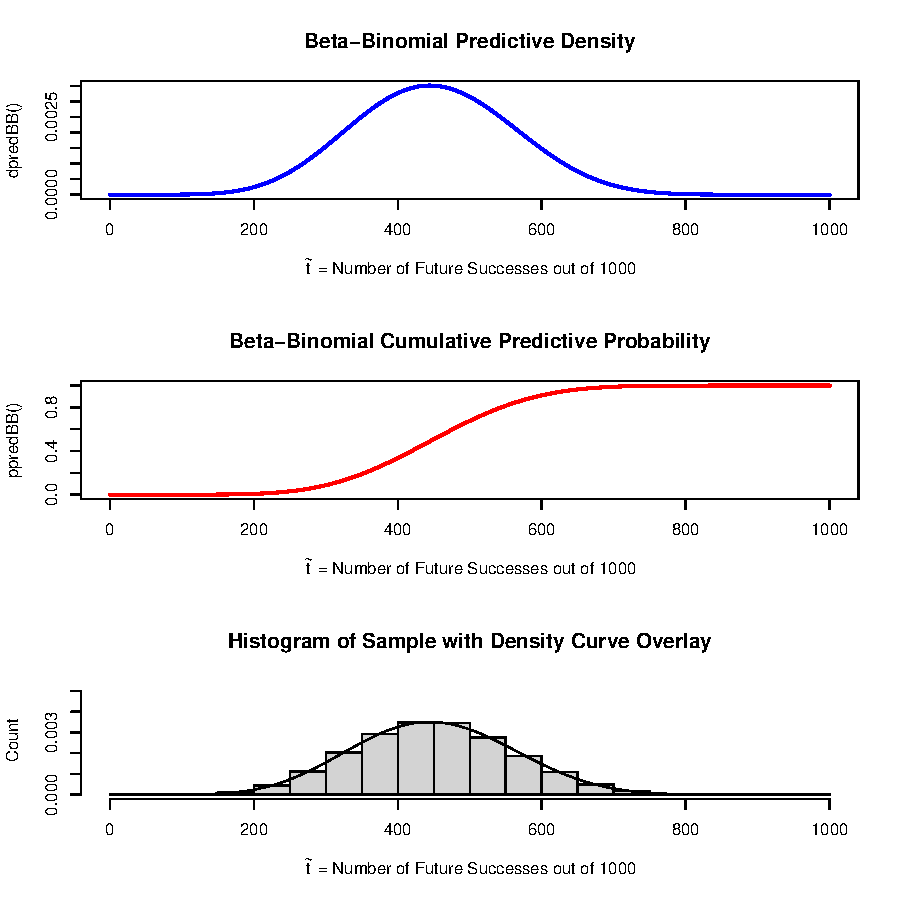
\includegraphics{Thesis_v4-003}



    \subsection{Survival Time:  Exponential-Gamma (Geisser p. 74)}

    \subsubsection{Derivation}

Suppose $Y_1,...,Y_d$ represent fully observed realizations from an exponential survival time density
          $$p(y|\theta) = \theta e^{-\theta y}$$
      and $Y_{d+1},...,Y_N$ represent censored copies surviving beyond the experimental time limit.  We assume $Y_1,...,Y_d$ are exchangeable and therefore conditionally i.i.d. with respect to $\theta$.\\

\noindent The usual exponential likelihood is used for the fully observed copies, whereas for the censored copies we need Pr$(Y > y | \theta) = 1 - \text{Pr}(Y\leq y | \theta) = 1 - F(y|\theta) = 1 - (1 - e^{-\theta y}) = e^{-\theta y}$.  Here $F$ denotes the cumulative distribution function.\\

\noindent Thus, with $\bar{y} = \frac{1}{N}\sum_{i=1}^N y_i$, the overall likelihood is

      $$L(\theta|y) = \prod_{i=1}^d\theta e^{-\theta y_i}\prod_{i=d+1}^N e^{-\theta y_i} = \theta^d e^{-\theta N\bar{y}}$$

\noindent Assuming a Gamma$(\delta,\gamma)$ prior for $\theta$,

       $$\pi(\theta) = \frac{\gamma^\delta\theta^{\delta - 1}e^{-\gamma\theta}}{\Gamma(\delta)}$$

\noindent we obtain the posterior

        \begin{flalign*}
          p(\theta|Y_1,...,Y_N)
          &= \frac{p(Y_1,...,Y_N|\theta)\pi(\theta)}{\int p(Y_1,...,Y_N|\theta)\pi(\theta)d\theta}\\
          &\\
          &= \frac{\theta^d e^{-\theta N\bar{y}}\cdot\frac{\gamma^\delta\theta^{\delta - 1}e^{-\gamma\theta}}{\Gamma(\delta)}}{\int\left(\theta^d e^{-\theta N\bar{y}}\cdot\frac{\gamma^\delta\theta^{\delta - 1}e^{-\gamma\theta}}{\Gamma(\delta)}\right)d\theta}\\
          &\\
          &= \frac{\left(\theta^{d+\delta - 1}e^{-\theta(\gamma+N\bar{y})}\right)}{\int\left(\theta^{d+\delta - 1}e^{-\theta(\gamma+N\bar{y})}\right)d\theta}\\
          &\\
          &= \frac{(\gamma+N\bar{y})^{d+\delta}}{\Gamma(d+\delta)}\theta^{d+\delta - 1}e^{-\theta(\gamma+N\bar{y})}\\
          &\\
          &=\text{Gamma}(d+\delta,\gamma+N\bar{y}),
        \end{flalign*}

\noindent with the Gamma$(d+\delta,\gamma+N\bar{y})$ density in the denominator of next to last step integrating to $1$.\\

\noindent The survival time predictive probability density then is

    \begin{flalign}
      p(\tilde{y}|Y_1,...,Y_N)
      &= \int p(\tilde{y}|\theta)p(\theta|y_1,...,y_N)d\theta\nonumber\\
      &\nonumber\\
      &= \int \theta e^{-\theta \tilde{y}} \cdot \frac{(\gamma+N\bar{y})^{d+\delta}\theta^{d+\delta - 1}e^{-\theta(\gamma+N\bar{y})}}{\Gamma(d+\delta)}d\theta\nonumber\\
      &\nonumber\\
      &= (d+\delta)(\gamma+N\bar{y})^{d+\delta}\int\frac{\theta^{(d+\delta + 1) - 1}e^{-\theta(\gamma+N\bar{y} + \tilde{y})}}{(d+\delta)\Gamma(d+\delta)}d\theta\nonumber\\
      &\nonumber\\
      &= \frac{(d+\delta)(\gamma+N\bar{y})^{d+\delta}}{\left(\gamma+N\bar{y}+\tilde{y}\right)^{d+\delta+1}}\int\frac{\left(\gamma+N\bar{y}+\tilde{y}\right)^{d+\delta+1}\theta^{(d+\delta + 1) - 1}e^{-\theta(\gamma+N\bar{y} + \tilde{y})}}{\Gamma(d+\delta+1)}d\theta\nonumber\\
      &\nonumber\\
      &= \frac{(d+\delta)(\gamma+N\bar{y})^{d+\delta}}{\left(\gamma+N\bar{y}+\tilde{y}\right)^{d+\delta+1}}\label{exponentialGamma_pred},
    \end{flalign}

\noindent simplifying here by constructing a Gamma$(d+\delta+1,\gamma+N\bar{y}+\tilde{y})$ density in the final integrand.\\



    \subsubsection{R Implementation (Exponential-Gamma)}

This result has been used to create R functions \texttt{dpredEG()}, \texttt{ppredEG()}, and \texttt{rpredEG()} for the Gamma-Exponential distribtuion for density, cumulative probability, and random sampling, respectively (see appendix for R code).  These functions are exercised in the following example. \\

\noindent The density function \texttt{dpredEG()} evaluates the numerator and denominator of the predictive density logarithmically (using the R function \texttt{log()}) and then exponentiates to produce the result.  The cdf \texttt{ppredEG()} integrates the pdf at each discrete value using the R function \texttt{integrate()}.  The random sampler \texttt{rpredEG()} draws posterior $\theta|y_1,...,y_i\sim\text{Gamma}(d+\delta,\gamma+\sum y_i)$ and then draws predictions from Exp$(\theta)$. Calls to these functions appear as follows:

\begin{center}
  \texttt{dpredEG(ypred,y,c,dt,gm)}\\
  \texttt{ppredEG(ypred,y,c,dt,gm)}\\
  \texttt{rpredEG(S,y,c,dt,gm)}\\
\end{center}

\noindent where

\begin{flalign*}
  \texttt{ypred} &= \tilde{y} \text{, the survival time(s) in future experiments for which prediction is desired}\\
  \texttt{y} &= \text{a vector of } N \text{ survival times, } d \text{ observed, } N-d \text{ censored}\\
  \texttt{c} &= \text{an indicator vector of length } N.\texttt{  c[i]=1}\text{ if the corresponding data element }\texttt{y[i]}\text{ is fully }\\ &\text{   observed, otherwise }\texttt{c[i]=0.}  \text{  Note }\texttt{d = sum(c).}\\
  \texttt{dt} &= \delta \text{, the shape parameter of the Gamma prior}\\
  \texttt{gm} &= \gamma \text{, the rate parameter of the Gamma prior}\\
  \texttt{S} &= \text{the desired random sample size}\\
\end{flalign*}


    \subsubsection{Example}

    \textcolor{red}{This needs updating.  Also, think about the number of new observations to be predicted.  Why would we (you) choose M=1000?}\\

\noindent Suppose $d=797$ out of $N = 1000$ copies have been observed, and the remaining $203$ censored. We are interested in the number of survivors out of $M = 1000$ future observations.  For the sake of this example, survival times were generated randomly as $y_i \sim \text{Exp}(0.01)$, with all times exceeding an arbitrary predetermined time cutoff of 160 being set to that time.  These reset times are the censored copies.  We know the value of the exponential parameter ($\theta = 0.01$) used to generate the data, because of the artificial way we have constructed this example.  If we did not have that information, we could consider the mean of the generated survival times (observed and censored), which was $79.9$.  This indicates that the expected value $1/\theta$ of survival times must be greater than $79.9$, and thus we can assume $\theta < 1/79.9 \approx 0.0125$ with some margin.  This is all to say that aiming for $\theta = 0.01$ when choosing parameters for the prior distribution of $\theta$ is reasonable.  Since we are assuming prior $\theta\sim\text{Gamma}(\delta,\gamma)$ we want $\delta/\gamma \approx 0.01$.   For this example, say $\delta = 0.5$ and $\gamma=50$.  The figures below illustrate the predictive probability using \texttt{dpredEG()} and \texttt{rpredEG()}, along with a histogram of a random sample taken using \texttt{rpredEG()}.



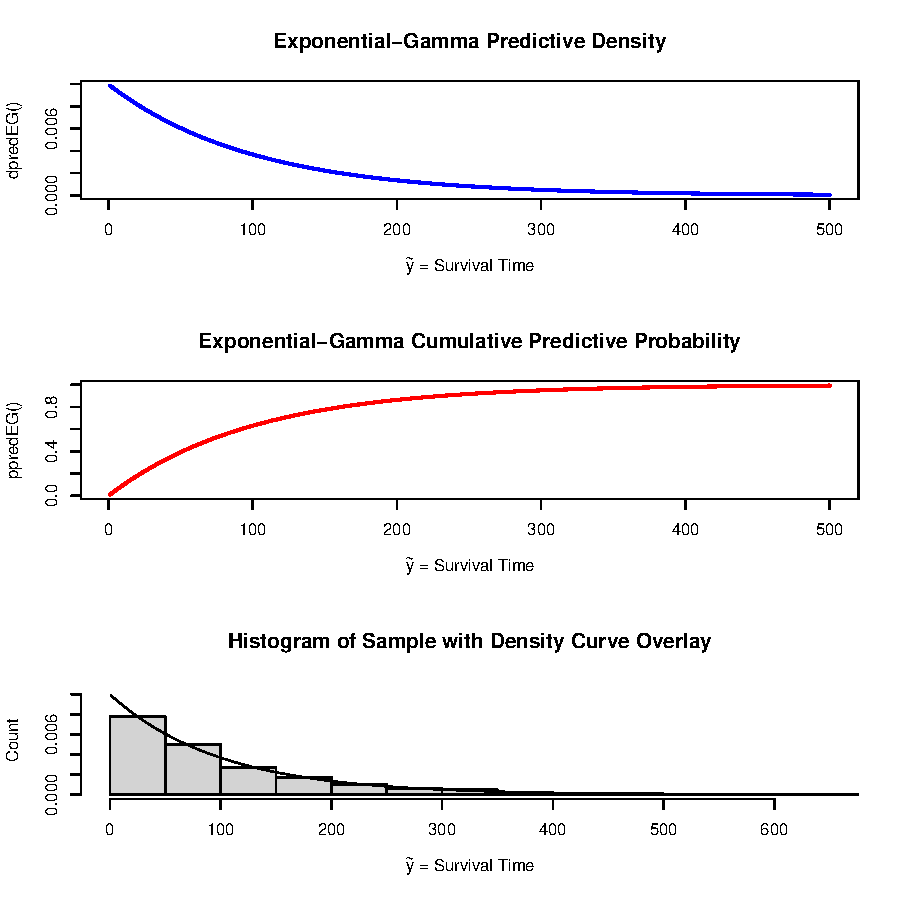
\includegraphics{Thesis_v4-004}


\clearpage

  \subsection{Poisson-Gamma Model (Hoff p. 43 - 50)}

    \subsubsection{Derivation}

      Suppose we have exchangeable count data observations $Y_1,...,Y_N|\theta\overset{i.i.d.}{\sim}\text{Poisson}(\theta)$, with $\theta$ assumed to have prior Gamma$(\alpha,\beta)$ distribution.  That is,

      \begin{flalign*}
        P\left(Y_1 = y_1,...,Y_N = y_N|\theta\right)
        &= \prod_{i=1}^N p\left(y_i|\theta\right)\\
        &\\
        &= \prod_{i=1}^N\frac{1}{y!}\theta^{y_i}e^{-\theta}\\
        &\\
        &= \left(\prod_{i=1}^N\frac{1}{y!}\right)\theta^{\sum y_i}e^{-N\theta}\\
        &\\
        &= c\left(y_1,...,y_N\right)\theta^{\sum y_i}e^{-N\theta}
      \end{flalign*}

\noindent and

      $$\pi(\theta) = \dfrac{\beta^\alpha}{\Gamma(\alpha)}\theta^{\alpha-1}e^{-\beta\theta} \text{ with } \theta, \alpha, \beta > 0.$$

\bigskip

\noindent Then we have posterior

      \begin{flalign*}
        p\left(\theta|y_1,...,y_N\right)
        &= \dfrac{p\left(y_1,...,y_N|\theta\right)\pi(\theta)}{\int_\theta p\left(y_1,...,y_N|\theta\right)p(\theta)d\theta}\\
        &\\
        &= \dfrac{p\left(y_1,...,y_N|\theta\right)\pi(\theta)}{p\left(y_1,...,y_N\right)}\\
        &\\
        &= \dfrac{1}{p\left(y_1,...,y_N\right)}\theta^{\sum y_i}e^{-N\theta}\dfrac{\beta^\alpha}{\Gamma(\alpha)}\theta^{\alpha - 1}e^{-\beta\theta}\\
        &\\
        &= C\left(y_1,...,y_N,\alpha,\beta\right)\theta^{\alpha+\sum y_i - 1}e^{-(\beta + N)\theta}\\
        &\\
        &\propto \text{Gamma}\left(\alpha+\sum y_i,\beta + N\right).
      \end{flalign*}

\noindent Here

      \begin{flalign*}
        C\left(y_1,...,y_N,\alpha,\beta\right)
        &= \dfrac{1}{p\left(y_1,...,y_N\right)}\cdot\dfrac{\beta^\alpha}{\Gamma(\alpha)}\\
        &\\
        &= \dfrac{1}{\int_\theta p\left(y_1,...,y_N|\theta\right)\pi(\theta)d\theta}\cdot\dfrac{\beta^\alpha}{\Gamma(\alpha)}\\
        &\\
        &= \dfrac{1}{\int_\theta\left(\prod\frac{1}{y_i!}\right)\theta^{\sum y_i}e^{-N\theta}\cancel{\left(\frac{\beta^\alpha}{\Gamma(\alpha)}\right)}\theta^{\alpha-1}e^{-\beta\theta}d\theta}\cdot\cancel{\left(\frac{\beta^\alpha}{\Gamma(\alpha)}\right)}
        &\\
        &= \dfrac{1}{\left(\prod\frac{1}{y_i!}\right)\frac{\Gamma(\alpha + \sum y_i)}{(\beta+N)^{\alpha+\sum y_i}}\int_\theta \frac{(\beta+N)^{\alpha+\sum y_i}}{\Gamma(\alpha+\sum y_i)}\theta^{\sum y_i+\alpha-1}e^{-(\beta+N)\theta}d\theta}\\
        &\\
        &= \dfrac{\prod_{i=1}^N y_i!(\beta+N)^{\alpha+\sum y_i}}{\Gamma(\alpha+\sum y_i)}
      \end{flalign*}

\noindent Call this constant $C_N$ (for $N$ observations).

\bigskip

\noindent Note that with an additional observation $\tilde{y} = y_{N+1}$ the constant becomes

      $$C_{N+1} = \dfrac{\prod_{i=1}^{N+1} y_i!(\beta+N+1)^{\alpha+\sum_{i=1}^{N+1} y_i}}{\Gamma(\alpha+\sum_{i=1}^{N+1} y_i)}.$$

\noindent Also note that the marginal joint distribution of $k$ observations is

      $$p(y_1,...,y_k) = \dfrac{1}{C_k}\dfrac{\beta^\alpha}{\Gamma(\alpha)}.$$

\noindent For future observation $\tilde{y}$, then, we compute predictive distribution

      \begin{flalign}
        p\left(\tilde{y}|y_1,...,y_N\right)
        &= \dfrac{p\left(y_1,...,y_N,\tilde{y}\right)}{p\left(y_1,...,y_N\right)} = \dfrac{p\left(y_1,...,y_{N+1}\right)}{p\left(y_1,...,y_N\right)}
        = \dfrac{\frac{1}{C_{N+1}}\cancel{\frac{\beta^\alpha}{\Gamma(\alpha)}}}{\frac{1}{C_N}\cancel{\frac{\beta^\alpha}{\Gamma(\alpha)}}}
        = \dfrac{C_N}{C_{N+1}}\nonumber\\
        &\nonumber\\
        &= \dfrac{\dfrac{\prod_{i=1}^N y_i!(\beta+N)^{\alpha+\sum_{i=1}^N y_i}}{\Gamma(\alpha+\sum_{i=1}^N y_i)}}{\dfrac{\prod_{i=1}^{N+1} y_i!(\beta+N+1)^{\alpha+\sum_{i=1}^{N+1} y_i}}{\Gamma(\alpha+\sum_{i=1}^{N+1} y_i)}}\nonumber\\
        &\nonumber\\
        &= \dfrac{\Gamma\left(\alpha+\sum_{i=1}^{N+1}y_i\right)(\beta+N)^{\alpha+\sum_{i=1}^N y_i}}{\left(y_{N+1}!\right)\Gamma\left(\alpha+\sum_{i=1}^N y_i\right)(\beta+N+1)^{\alpha+\sum_{i=1}^{N+1}y_i}}\nonumber\\
        &\nonumber\\
        &= \dfrac{\Gamma\left(\alpha+\sum_{i=1}^N y_i + \tilde{y}\right)(\beta+N)^{\alpha+\sum_{i=1}^N y_i}}{\left(\tilde{y}!\right)\Gamma\left(\alpha+\sum_{i=1}^N y_i\right)(\beta+N+1)^{\alpha+\sum_{i=1}^N y_i + \tilde{y}}}\nonumber\\
        &\nonumber\\
        &= \dfrac{\Gamma\left(\alpha+\sum y_i+\tilde{y}\right)}{\Gamma(\tilde{y}+1)\Gamma(\alpha+\sum y_i)}\cdot \left(\dfrac{\beta+N}{\beta+N+1}\right)^{\alpha+\sum y_i} \cdot \left(\dfrac{1}{\beta+N+1}\right)^{\tilde{y}}\label{poissonGamma_pred}
      \end{flalign}

\noindent This is a negative binomial distribution:  $\tilde{y}\sim\text{NB}\left(\alpha+\sum y_i,\beta+N\right)$





    \subsubsection{R Implementation (Poisson-Gamma)}

This result has been used to create R functions \texttt{dpredPG()}, \texttt{ppredPG()}, and \texttt{rpredPG()} for the Poisson-Gamma distribution for density, cumulative probability, and random sampling, respectively (see appendix for R code).  These functions are exercised in the example below.\\

\noindent The density function \texttt{dpredPG()} simply makes use of the R function \texttt{dnbinom()}.  The cdf \texttt{ppredPG()} returns a cumulative sum of the results of \texttt{dpredPG()}.  The random sampler \texttt{rpredPG()} is a bit more complicated. The difficulty is that the upper bound of the support of the predictive distribution $p(\tilde{y}|y_1,...,y_n)$ is not known.  Since $p(\cdot)$ is negative binomial, we can count on it eventually decreasing toward $0$ asymptotically.  To establish the support, then, a method was employed to find where $p$ comes ``sufficiently close" to $0$.  To accomplish this a modified bisection method was devised as follows:\\

% Initially the R function \texttt{uniroot()} was considered, but ultimately a modified bisection method was devised as follows:\\

    \begin{enumerate}
      \item Set a desired tolerance $\epsilon$ for the distance of the predictive distribution above zero at the upper end of its support.  Currently the function leverages the local device's numerical precision with $\epsilon = $ \texttt{sqrt(.Machine\$double.eps)}.
      \item Set lower endpoint $L$ equal to the expected value of $\tilde{Y}$.  That is, $L = E(\tilde{Y}|y_1,...,y_N) = \dfrac{\alpha+\sum{y_i}}{\beta+N}$ (negative binomial). % L is not likely to be an integer, which doesn't matter, because L will not be fed back into the NB distribution
      \item Step to the right of $L$ by increments in the sequence $\{L+2^k:k=1,2,...\}$, setting upper endpoint $U_{test} = L+2^k$ using the first value of $k$ for which $\texttt{dpredPG}\left(L + 2^k\right) < 0$.
      \item Bisect $[L,U_{test}]$ letting $B$ be the integer nearest to the middle of the interval.
      \item Test whether $0 \leq \texttt{dpredPG}(B) \leq \epsilon$.  If so, accept $U = B$ as the upper end of the support.  If not:
      \item Establish a new interval $[L',U'_{test}]$ as follows:
      \begin{enumerate}
        \item if $[\texttt{dpredPG}(L),\texttt{dpredPG}(B)]$ straddles $0$, then $[L',U'_{test}] = [L,B]$.
        \item if $[\texttt{dpredPG}(B),\texttt{dpredPG}(U_{test})]$ straddles $0$, then $[L',U'_{test}] = [B,U_{test}]$.
      \end{enumerate}
      \item Repeat steps 3 - 5 above with the updated interval $[L,U_{test}] = [L',U'_{test}]$ until the condition in step 5 is reached, establishing upper bound $U$.
      \item Use $[0,U]$ as the support upon which to draw a random sample.
    \end{enumerate}


\noindent Calls to these functions appear as follows:

\begin{center}
  \texttt{dpredPG(ypred,y,alpha,beta)}\\
  \texttt{ppredPG(ypred,y,alpha,beta)}\\
  \texttt{rpredPG(S,y,alpha,beta)}\\
\end{center}

\noindent where

\begin{flalign*}
  \texttt{ypred} &= \tilde{y} \text{, future count(s) for which prediction is desired}\\
  \texttt{y} &= y \text{, the observed counts}\\
  \texttt{alpha} &= \alpha \text{, the shape parameter of the Gamma prior}\\
  \texttt{beta} &= \beta \text{, the rate parameter of the Gamma prior}\\
  \texttt{S} &= S \text{, the desired random sample size}\\
\end{flalign*}

    \subsubsection{Example}

\textcolor{red}{I will come up with a different example to replace the one below.}

Suppose we have 10 prior observations with counts 27, 79, 21, 100, 8, 4, 37, 15, 3, 97.  Let $\alpha = 11$ and $\beta = 3$.  For $\tilde{y} = 1:100$ possible future occurrences, the figures below show the predictive distribution from \texttt{dpredPG()}, the cumulative distribution from \texttt{ppredPG()}, and a histogram of random draws from \texttt{rpredPG()}.


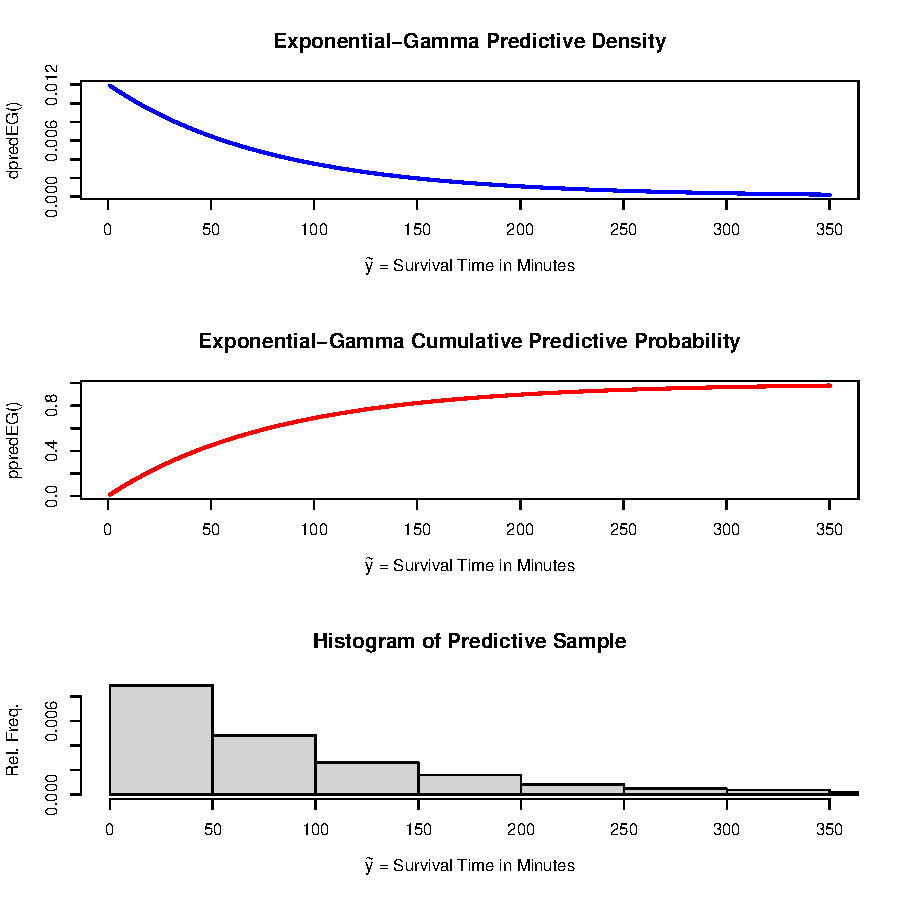
\includegraphics{Thesis_v4-005}



\clearpage

  \subsection{Normal Observation with Normal-Inverse Gamma Prior}

    \subsubsection{One sample Normal-Inverse Gamma}
      \paragraph{Derivation} (Hoff Ch. 5)

\noindent Let $\left\{Y_1,...,Y_N|\theta,\sigma^2\right\}\overset{i.i.d.}{\sim}\text{Normal}\left(\theta,\sigma^2\right)$ (assuming $Y_1,...,Y_N$ are exchangeable).  Then the joint sampling density is

        \begin{flalign*}
          p\left(y_1,...,y_N|\theta,\sigma^2\right)
          &= \prod_{i=1}^N p\left(y_i|\theta,\sigma^2\right)\\
          &\\
          &= \prod_{i=1}^N \dfrac{1}{\sqrt{2\pi\sigma^2}}e^{-\frac{1}{2}\left(\frac{y_i - \theta}{\sigma}\right)^2}\\
          &\\
          &= \left(2\pi\sigma^2\right)^{-\sfrac{N}{2}}e^{-\frac{1}{2}\sum_{i=1}^N\left(\frac{y_i - \theta}{\sigma}\right)^2}.\\
        \end{flalign*}

\noindent Following Hoff (p. 74-75), for joint inference on both $\theta$ and $\sigma$, we assign priors

        \begin{flalign*}
          \frac{1}{\sigma^2} &\sim \text{Gamma}\left(\sfrac{\nu_0}{2},\sfrac{\nu_0\sigma_0^2}{2}\right)\\
          &\\
          \theta|\sigma^2 &\sim \text{Normal}\left(\mu_0,\sfrac{\sigma^2}{\kappa_0}\right)\\
        \end{flalign*}

\noindent Hoff suggests $\sigma_0^2$ and $\nu_0$ can be interpreted heuristically as sample variance and sample size, respectively, of prior observations, and that  $\mu_0$ and $\kappa_0$ can be thought of as the sample mean and sample size of prior observations.\\

\noindent From this we derive joint posterior distribution

        \begin{flalign*}
          \left\{\theta|y_1,...,y_N,\sigma^2\right\} &\sim \text{Normal}\left(\mu_N,\sfrac{\sigma^2}{\kappa_N}\right)\\
          &\\
          \left\{\sigma^2|y_1,...,y_N\right\} &\sim \text{Inverse Gamma}\left(\sfrac{\nu_N}{2},\sfrac{\sigma^2_N\nu_N}{2}\right).
        \end{flalign*}

\noindent where

        \begin{flalign*}
          \kappa_N &= \kappa_0 + N\\
          &\\
          \mu_N &= \frac{\kappa_0\mu_0+N\bar{y}}{\kappa_N}\\
          &\\
          \nu_n &= \nu_0 + N\\
          &\\
          \sigma_N^2 &= \frac{1}{\nu_N}\left[\nu_0\sigma_0^2 + (N-1)s^2 + \frac{\kappa_0 N}{\kappa_N}\left(\bar{y}-\mu_0\right)^2\right].\\
        \end{flalign*}

\noindent Here $\bar{y} = \frac{1}{N}\sum_{i=1}^N y_i$ is the sample mean and $s^2 = \frac{1}{N-1}\sum_{i=1}^N\left(y_i - \bar{y}\right)^2$ is the sample variance.\\

\noindent From the joint posterior distribution we generate marginal samples by means of the monte carlo method (Hoff, p. 77):

        \begin{flalign*}
          \begin{matrix}
            \sigma^{2(1)}\sim \text{Inverse Gamma}\left(\nu_N/2,\sigma^2_N\nu_N/2\right), & \theta^{(1)}\sim \text{Normal}\left(\mu_N,\sigma^{2(1)}/\kappa_N\right) \\
            \vdots  & \vdots  \\
            \sigma^{2(S)}\sim \text{Inverse Gamma}\left(\nu_N/2,\sigma^2_N\nu_N/2\right), & \theta^{(S)}\sim \text{Normal}\left(\mu_N,\sigma^{2(S)}/\kappa_N\right) \\
          \end{matrix}
        \end{flalign*}

\noindent For prediction of future $\tilde{y}|y_1,...,y_N,\theta,\sigma^2$, generate $\tilde{y}_i \sim \text{Normal}\left(\theta^{(i)},\sigma^{2(i)}\right)$.\\

\noindent For prediction without the influence of any previous knowledge (Hoff p. 79), we can employ Jeffreys prior $\tilde{p}\left(\theta,\sigma^2\right) = 1/\sigma^2$.  This leads to the same conditional distribution for $\theta$ but a gamma$\left(\frac{N-1}{2},\frac{1}{2}\sum\left(y_i - \bar{y}\right)^2\right)$ distribution for $1/\sigma^2$.  This joint posterior distribution can be used to predict future $\tilde{y}$ by first drawing $\theta,\sigma^2$ and then simulating $\tilde{y}\sim\text{Normal}\left(\theta,\sigma^2\right)$.   Alternatively, the joint posterior can be integrated to show that
        $$\dfrac{\theta-\bar{y}}{s/\sqrt{N}}|y_1,...,y_N\sim t_{N-1}.$$
\noindent The resulting predictive distribution for $\tilde{y}$ is a t-distribution with location $\bar{y}$ and scale $s\sqrt{1+1/N}$ and $N-1$ degrees of freedom (Gelman et. al. p. 66).


      \paragraph{R Implementation (Normal-Inverse Gamma, 1-sample)}
      R functions \texttt{dpredNormIG1()}, \texttt{ppredNormIG1()}, and \texttt{rpredNormIG1()} have been created for the Normal-Inverse Gamma distribution for density, cumulative probability, and random sampling, respectively (see appendix).  These functions all include options for implementation with or without previous knowledge as desired.  If Jeffreys prior is used, the functions simply implement R's Student's t-distribution functions \texttt{rt()}, \texttt{dt()}, and \texttt{pt()}, applying the location and scale parameters as described above.  For predictions using previous knowledge, the functions work as follows:  For the random sampler \texttt{rpredNormIG1()}, the monte carlo method described above is directly employed.  The predictive density and cumulative predictive density functions (\texttt{dpredNormIG1()} and \texttt{ppredNormID1()}, respectively) depend on the random sample. That is, the distributions generated by these two functions are approximated from a random sample returned by \texttt{rpredNormIG1()}.\\

\noindent\texttt{ppredNormIG1()} utilizes the empirical cumulative density function \texttt{ecdf()} from R's stats package.  \texttt{dpredNormIG1()} utilizes a Kernel Density Estimation (KDE) method and R's built-in \texttt{density()} function.  The KDE is computed by definition, using a Normal kernel:

      $$\hat{f}_K(x) = \frac{1}{N}\sum_{i=1}^N\frac{1}{h}K\left(\frac{x-X_i}{h}\right),$$

\noindent where

      \begin{flalign*}
        X_i & \text{ is the random sample generated using }\texttt{rpredNormIG1()}\\
        &\\
        K & \text{ is Normal}(0,1)\\
        &\\
        h & \text{ is the bandwidth from R's }\texttt{density()}\text{ function (that is, } \texttt{h = density(X}_\texttt{i}\texttt{)\$bw)}\\
      \end{flalign*}

Calls to these functions appear as follows:

\begin{center}
  \texttt{dpredNormIG1(ypred,y,mu0,k0,sig20,nu0,S,Jeffreys)}\\
  \texttt{ppredNormIG1(ypred,y,mu0,k0,sig20,nu0,S,Jeffreys)}\\
  \texttt{rpredNormIG1(S,y,mu0,k0,sig20,nu0,Jeffreys)}\\
\end{center}

\noindent where

\begin{flalign*}
  \texttt{ypred} &= \tilde{y} \text{, value(s) for which prediction is desired}\\
  \texttt{y} &= \mathbf{y} \text{, the observed data}\\
  \texttt{mu0} &= \mu_0 \text{, prior parameter for }\theta\text{, representing the mean of prior observations}\\
  \texttt{k0} &= \kappa_0 \text{, prior parameter for }\theta\text{, representing the sample size of prior observations}\\
  \texttt{sig20} &= \sigma^2_0 \text{, prior parameter for }\sigma^2\text{, representing the variance of prior observations}\\
  \texttt{nu0} &= \nu_0 \text{, prior parameter for }\sigma^2\text{, representing the sample size of prior observations}\\
  \texttt{S} &= S \text{, the desired number of predictions to be generated}\\
  \texttt{Jeffreys} &= \text{ flag (defaulting to }\texttt{FALSE}\text{), controlling the decision to use Jeffrey's prior}
\end{flalign*}


\noindent These functions are exercised in the following example.\\


      \paragraph{Example}

        \textit{Example (Hoff p. 72ff, using data from Grogan and Wirth (1981)):  Midge wing length}\\

        Grogan and Wirth (1981) provide 9 measurements of midge wing length, in millimeters:  $y = \{1.64, 1.7, 1.72, 1.74, 1.82, 1.82, 1.82, 1.90, 2.08\}$. Previous studies suggest values $\mu_0 = 1.9$ and $\sigma_0^2 = 0.01$.  We choose $\kappa_0 = \nu_0 = 1$ ``...so that our prior distributions are only weakly centered around these estimates from other populations" (Hoff p. 76). We compute

        \begin{flalign*}
          \bar{y} &= 1.804\\
          &\\
          \text{var}(y) &= 0.0169\\
          &\\
          \kappa_N &= 1 + 9 = 10\\
          &\\
          \mu_N &= \frac{1 \cdot 1.9 + 9 \cdot 1.804}{10} = 1.814\\
          &\\
          \nu_N &= 1 + 9 = 10\\
          &\\
          \sigma_N^2 &= \frac{1}{10}\left[1 \cdot 0.01 + (9-1) \cdot 0.0169 + \frac{1 \cdot 9}{10}\left(1.804 - 1\right)^2\right] = 0.0153\\
        \end{flalign*}

\noindent Thus $\sfrac{\nu_N}{2} = 5$ and $\sfrac{\nu_N\sigma_N^2}{2} = 0.7662$ and we have posteriors

        \begin{flalign*}
          \left\{\theta|y_1,...,y_N,\sigma^2\right\} &\sim \text{Normal}\left(1.814,\sfrac{\sigma^2}{10}\right)\\
          &\\
          \left\{\sigma^2|y_1,...,y_N\right\} &\sim \text{Inverse Gamma}(5,0.7662)\\
        \end{flalign*}

\noindent The plot below illustrates the influence of previous knowledge of the population mean, and compares to the predictions resulting from Jeffreys prior.

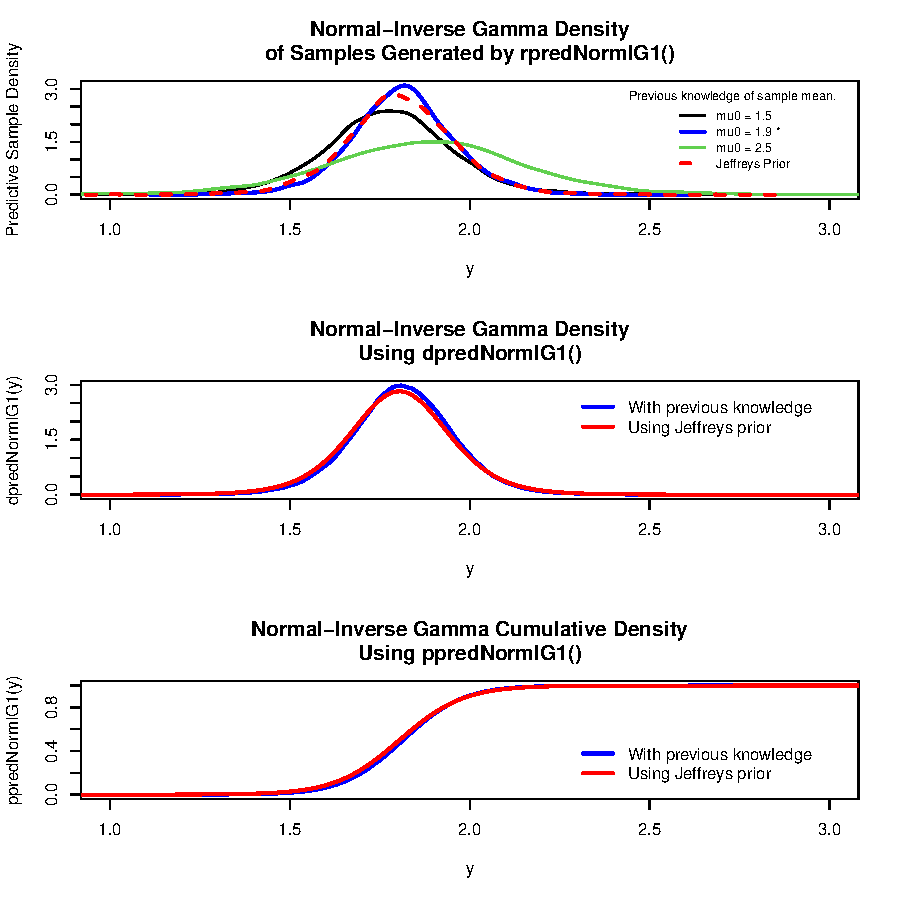
\includegraphics{Thesis_v4-006}

\noindent Clearly the prediction relying on prior knowledge heavily depends on the the quality of that prior knowledge.  Jeffrey's prior in this case produces results close to the case where the supplied prior mean is more informed.  \textcolor{blue}{Feedback on this paragraph?}

        \clearpage

    \subsubsection{Two-sample Normal-Inverse Gamma}
      \paragraph{Derivation}

        For a Bayesian analysis comparing two exchangeable groups $Y_{1,1},...,Y_{N_1,1}$ and $Y_{1,2},...,Y_{N_2,2}$ we use the following sampling model (Hoff p. 127):

        \begin{flalign*}
          Y_{i,1} &= \mu + \delta + \epsilon_{i,1}\\
          Y_{i,2} &= \mu - \delta + \epsilon_{i,2}\\
          \left\{\epsilon_{i,j}\right\} &\sim\text{i.i.d. Normal}\left(0,\sigma^2\right).
        \end{flalign*}

\noindent Letting $\theta_1 = \mu + \delta$ and $\theta_2 = \mu - \delta$ we see that $\delta = \left(\theta_1 - \theta_2\right)/2$ is half the population difference in means, and $\mu = \left(\theta_1 + \theta_2\right)/2$ is the pooled average.  We'll assume conjugate prior distributions

        \begin{flalign*}
          \pi\left(\mu,\delta,\sigma^2\right) &= \pi(\mu) \times \pi(\delta) \times \pi\left(\sigma^2\right)\\
          \mu &\sim \text{Normal}\left(\mu_0,\gamma^2_0\right)\\
          \delta &\sim \text{Normal}\left(\delta_0,\tau^2_0\right)\\
          \sigma^2 &\sim \text{Inverse Gamma}\left(\nu_0/2,\nu_0\sigma^2_0/2\right).
        \end{flalign*}

\noindent Here $\nu_0$ as before represents the prior sample size.   The full conditional distributions follow:\\

        \indent $\left\{\mu|\mathbf{y}_1,\mathbf{y}_2,\delta,\sigma^2\right\} \sim \text{Normal}\left(\mu_N,\gamma^2_N\right)$, where

        \begin{flalign*}
          \mu_N &= \gamma^2_N \times \left[\dfrac{\mu_0}{\gamma^2_0} + \dfrac{\sum_{i=1}^{N_1}\left(y_{i,1}-\delta\right) + \sum_{i=1}^{N_2}\left(y_{i,2}+\delta\right)}{\sigma^2}\right]\\
          &\\
          \gamma^2_N &=\left[\dfrac{1}{\gamma^2_0} + \dfrac{\left(N_1 + N_2\right)}{\sigma^2}\right]^{-1}
        \end{flalign*}

        \indent $\left\{\delta|\mathbf{y}_1,\mathbf{y}_2,\mu,\sigma^2\right\} \sim \text{Normal}\left(\delta_N,\tau^2_N\right)$, where

        \begin{flalign*}
          \delta_N &= \tau^2_N \times \left[\dfrac{\delta_0}{\tau^2_0} + \dfrac{\sum_{i=1}^{N_1}\left(y_{i,1}-\mu\right) - \sum_{i=1}^{N_2}\left(y_{i,2}-\mu\right)}{\sigma^2}\right]\\
          &\\
          \tau^2_N &=\left[\dfrac{1}{\tau^2_0} + \dfrac{\left(N_1 + N_2\right)}{\sigma^2}\right]^{-1}
        \end{flalign*}

        \indent $\left\{\sigma^2|\mathbf{y}_1,\mathbf{y}_2,\mu,\delta\right\} \sim \text{Inverse Gamma}\left(\frac{\nu_N}{2},\frac{\nu_N\sigma^2_N}{2}\right)$, where

        \begin{flalign*}
          \nu_N &= \nu_0 + N_1 + N_2\\
          \\
          \nu_N\sigma^2_N &= \nu_0\sigma^2_0 + \sum_{i=1}^{N_1}\left(y_{i,1} - [\mu + \delta]\right)^2 + \sum_{i=1}^{N_2}\left(y_{i,2} - [\mu - \delta]\right)^2\\
        \end{flalign*}



      \paragraph{R Implementation (Normal-Inverse Gamma, 2-sample)}

      The random sample generator R function \texttt{rpredNormIG2()} implements a Gibbs sampler to approximate the posterior distribution $p\left(\mu,\delta,\sigma^2|\mathbf{y}_1,\mathbf{y}_2\right)$, from which to generate predictions for the two populations as follows:
      \begin{enumerate}
        \item Set initial values $\mu = \frac{\theta_1 + \theta_2}{2}$ and $\delta = \frac{\theta_1 - \theta_2}{2}$
        \item Generate a single $\sigma^2|\mathbf{y_1},\mathbf{y_2},\mu,\delta$
        \item Generate a single $\mu|\mathbf{y_1},\mathbf{y_2},\delta,\sigma^2$
        \item Generate a single $\delta|\mathbf{y_1},\mathbf{y_2},\mu,\sigma^2$
        \item Predict $\tilde{y}_1\sim \text{Normal}\left(\mu+\delta,\sigma^2\right)$ and $\tilde{y}_2\sim \text{Normal}\left(\mu-\delta,\sigma^2\right)$
      \end{enumerate}

\noindent The user provides the two samples $\mathbf{y_1}$ and $\mathbf{y_2}$ along with values for $\mu_0, \sigma^2_0, \delta_0, \tau^2_0, \nu_0$, and desired prediction random sample size $S$.  The function returns $S$ predictions for each population and the vectors of generated values for $\mu$, $\delta$, and $\sigma^2$.  Calls to this functions appear as follows:


\begin{center}
  \texttt{rpredNormIG2(S,y1,y2,mu0,g20,d0,t20,nu0,s20)}\\
\end{center}

\noindent where

\begin{flalign*}
  \texttt{S} &= S \text{, the desired random sample size}\\
  \texttt{y1, y2} &= \mathbf{y_1, y_2} \text{, the two sets of observed data}\\
  \texttt{mu0,g20} &= \mu_0,\gamma^2_0 \text{, prior mean and variance for }\mu\\
  \texttt{d0,t20} &= \delta,\tau^2_0 \text{, prior mean and variance for }\delta\\
  \texttt{nu0,s20} &= \nu_0,\sigma^2_0 \text{, prior parameters for the variance of the Normal data error terms}\\
\end{flalign*}

      \paragraph{Example} (Hoff p. 128-129 \textit{Analysis of math score data})\\
      Hoff provides the following example, which we reproduce here.\\\\
      Math score data for two public high schools in the United States (we'll call them School 1 and School 2) were based on results of a national exam, standardized to produce a nationwide mean of 50 and a standard deviation of 10.  The data consisted of 31 individual scores for School 1 and 28 for School 2. The plots below show give a visual summary of the two data sets.

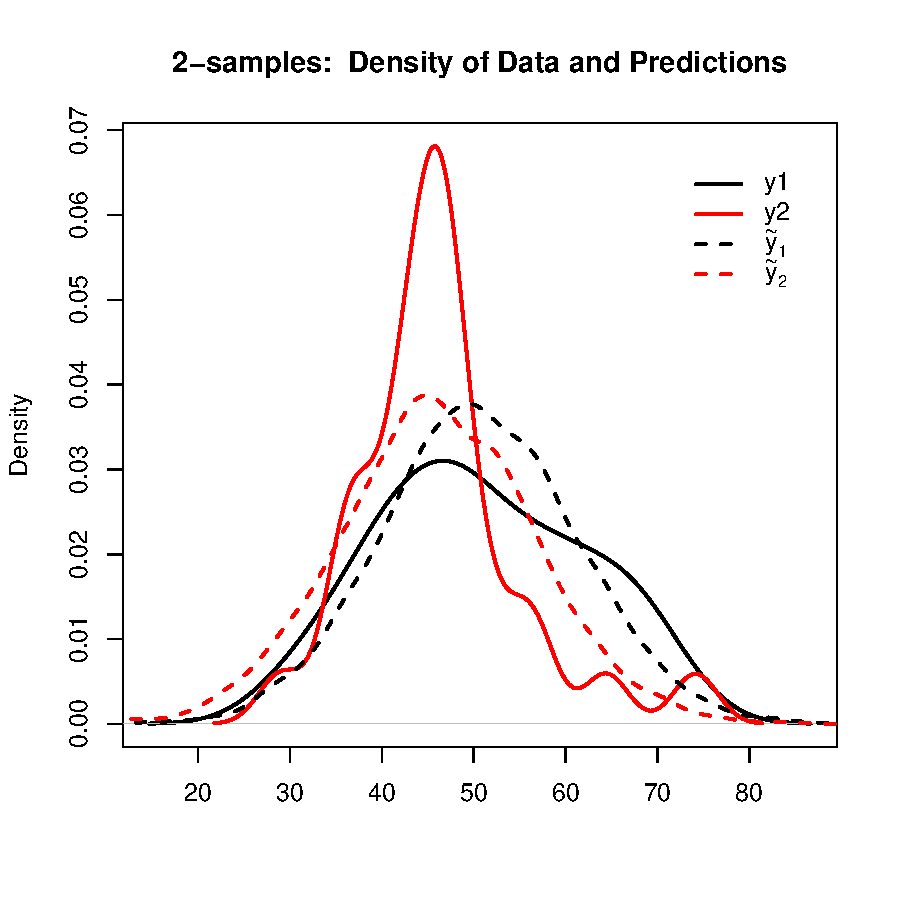
\includegraphics{Thesis_v4-007}

\noindent The mean scores of the two samples are $\bar{y}_1 = 50.81$ and $\bar{y}_2 = 46.15$ for School 1 and School 2, and the standard deviations were $11.3$ and $9.1$, respectively.  A standard t-test yields a $p$-value of $p = 0.087$, in response to which we would fail to reject the hypothesis that the population means $\theta_1$ and $\theta_2$ are different. Hoff points out that it is easy to imagine that re-sampling might result in a few more low scores from School 1 and a few more high scores from School 2--enough perhaps to result in a $p$-value below $0.05$ and the opposite conclusion. Why not employ a Bayesian analysis that allows information to be shared across the groups and relies on prior knowledge of the similarities of the two groups?\\

\noindent We're interested in predicting a future math score by a student from each school.  Unless the two schools were known in advance to be extremely exceptional, reasonable prior parameters can be based on this information.  For the prior distributions of $\mu$ and $\sigma^2$, we'll take $\mu_0 = 50$ and $\sigma^2_0 = 10^2 = 100$, although this latter value is likely to be an overestimate of the within-school sampling variability.  We'll make these prior distributions somewhat diffuse, with $\gamma^2_0 = 25^2 = 625$ and $\nu_0 = 1$.  For the prior distribution on $\delta$, choosing $\delta_0 = 0$ represents the prior opinion that $\theta_1 > \theta_2$ and $\theta_2 > \theta_1$ are equally probable.  Finally, since the scores are bounded between 0 and 100, half the difference between $\theta_1$ and $\theta_2$ must be less than 50 in absolute value, so a value of $\tau^2_0 = 25^2 = 625$ seems reasonably diffuse.\\\\

\textcolor{blue}{Anything else needed here? -- yes something below the plot describing the results.  Mention shared variance so data from different groups influencing each other.}
      % The results of a call to rpredNormIG2$\left(\mathbf{y}_1,\mathbf{y}_2,\mu_0,\sigma^2_0,\delta_0,\tau^2_0,N\right)$ are summarized in the following plot.\\
      The results of a call to \texttt{rpredNormIG2()} with the above input values for $\mathbf{y}_1,\mathbf{y}_2,\mu_0,\sigma^2_0,\delta_0,\tau^2_0,\text{ and } N$ are summarized in the following plot.\\

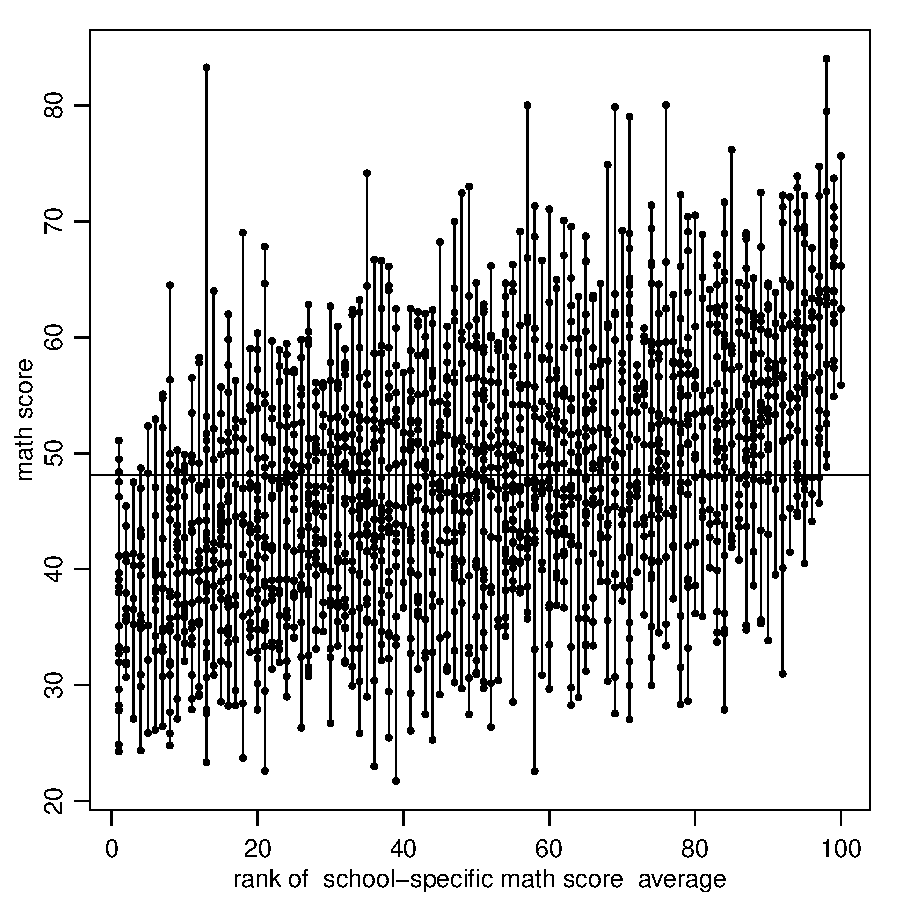
\includegraphics{Thesis_v4-008}


    \subsubsection{$k$-sample Normal-Inverse Gamma:  Comparing multiple groups}

    For two-level data consisting of groups and units within groups, denote data $\mathbf{Y}_1,...,\mathbf{Y_k}$ where $\mathbf{Y}_j = \{Y_{1,j},...,Y_{N_j,j}\}, j=1,...,k$. Here we stipulate exchangeability of $Y_{1,j},...,Y_{N_j,j}$, and thus we can model the data within group $j$ as conditionally i.i.d. given some parameter $\phi_j$.  We also assume that $\phi_1,...,\phi_k$ are exchangeable and thus conditionally i.i.d. given a parameter $\psi$, which has prior distribution $\pi(\psi)$.\\

\noindent We have the hierarchical Normal model (Hoff p. 132):
    $$\phi_j = \left\{\theta_j,\sigma^2\right\}, p\left(y|\phi_j\right) = \text{Normal}\left(\theta_j,\sigma^2\right) \text{ (within-group model)}$$
    $$\psi = \left\{\mu,\tau^2\right\}, p\left(\theta_j|\psi\right) = \text{Normal}\left(\mu,\tau^2\right) \text{ (between-groups model)}$$

\noindent We use standard semiconjugate Normal and Inverse Gamma prior distributions for the fixed but unknown parameters in the model:
    \begin{flalign*}
      \sigma^2 &\sim \text{Inverse Gamma}\left(\frac{\nu_0}{2},\frac{\nu_0\sigma^2_0}{2}\right)\\
      &\\
      \tau^2 &\sim \text{Inverse Gamma}\left(\frac{\eta_0}{2},\frac{\eta_0\tau^2_0}{2}\right)\\
      &\\
      \mu &\sim \text{Normal}\left(\mu_0,\gamma^2_0\right)\\
    \end{flalign*}

      \paragraph{Derivation}
      As with the two-sample problem, joint posterior inferences for the unknown parameters can be made by constructing a Gibbs sampler to approximate the posterior distribution $p\left(\theta_1,...,\theta_k,\mu,\tau^2,\sigma^2|\mathbf{y_1,...,y_k}\right)$.  For this we need the full conditional distribution of each parameter (Hoff pp. 134-135):
      $$\left\{\mu|\theta_1,...,\theta_k,\tau^2\right\} \sim \text{Normal}\left(\dfrac{\frac{k\bar{\theta}}{\tau^2} + \frac{\mu_0}{\gamma^2_0}}{\frac{k}{\tau^2} + \frac{1}{\gamma^2_0}},\dfrac{1}{\frac{k}{\tau^2}+\frac{1}{\gamma^2_0}}\right)$$
      $$\left\{\tau^2|\theta_1,...,\theta_k,\mu\right\} \sim \text{Inverse Gamma}\left(\dfrac{\eta_0 + k}{2},\dfrac{\eta_0\tau^2_0 + \sum\left(\theta_j-\mu\right)^2}{2}\right)$$

      $$\left\{\theta_j|y_{1,j},...,y_{n,j},\sigma^2\right\} \sim \text{Normal}\left(\dfrac{\frac{n_j\bar{y}_j}{\sigma^2} + \frac{1}{\tau^2}}{\frac{n_j}{\sigma^2}+\frac{1}{\tau^2}},\dfrac{1}{\frac{n_j}{\sigma^2}+\frac{1}{\tau^2}}\right)$$

      $$\left\{\sigma^2|\theta_1,...,\theta_k,\mathbf{y_1,...,y_k}\right\} \sim \text{Inverse Gamma}\left(\dfrac{1}{2}\left[\nu_0 + \sum_{j=1}^k n_j\right],\dfrac{1}{2}\left[\nu_0\sigma^2_0 + \sum_{j=1}^k\sum_{i=1}^{n_j}\left(y_{i,j}-\theta_j\right)^2\right]\right).$$

\noindent Here $\bar{\theta} = \frac{1}{k}\sum_{j=1}^k \theta_j$.  Note that $\sum\sum\left(y_{i,j}-\theta_j\right)^2$ is the sum of squared residuals across all groups, conditional on the within-group means, and so the conditional distribution concentrates probability around a pooled-sample estimate of the variance.\\

\noindent Finally, a prediction for the $j^{\text{th}}$ group is given by
$$\tilde{y}_j \sim \text{Normal}(\theta_j, \sigma^2).$$

      \paragraph{R Implementation (Normal-Inverse Gamma, k-samples)}

      The R function \texttt{rpredNormIGk()} implements a Gibbs sampler for posterior approximation of each unknown quantity by sampling from its full conditional distribution.  From these posteriors, predictions are generated, as follows:

      \begin{enumerate}
        \item Set prior parameter values:
          \begin{flalign*}
            \nu_0,\sigma^2_0 \text{ for } p\left(\sigma^2\right)\\
            \eta_0,\tau^2_0 \text{ for } p\left(\tau^2\right)\\
            \mu_0,\gamma^2_0 \text{ for } p\left(\mu\right).
          \end{flalign*}
        \item Set initial states for the unknown parameters:
          \begin{flalign*}
            \theta_1^{(1)} &= \mathbf{\bar{y}_1},...,\theta_k^{(1)} = \mathbf{\bar{y}_k}\\
            \mu^{(1)} &= \text{mean}\left(\theta_1^{(1)},...,\theta_k^{(1)}\right)\\
            \tau^{2(1)} &= \text{var}\left(\theta_1^{(1)},...,\theta_k^{(1)}\right)\\
            \sigma^{2(1)} &= \text{mean}\left(\text{var}\left(\mathbf{y}_1\right),...,\text{var}\left(\mathbf{y}_k\right)\right))
          \end{flalign*}
        \item For $s\in\{1,...,S\}$, sample
          \begin{enumerate}
            \item $\mu^{(s+1)} \sim p\left(\mu|\theta_1^{(s)},...,\theta_k^{(s)},\tau^{2(s)}\right)$
            \item $\tau^{2(s+1)} \sim p\left(\tau^2|\theta_1^{(s)},...,\theta_k^{(s)},\mu^{(s+1)}\right)$
            \item $\sigma^{2(s+1)} \sim p\left(\sigma^2|\theta_1^{(s)},...,\theta_k^{(s)},\mathbf{y}_1,...,\mathbf{y}_k\right)$
            \item $\theta_j^{(s+1)} \sim p\left(\theta_j|\mu^{(s+1)},\tau^{2(s+1)},\sigma^{2(s+1)},\mathbf{y}_j\right)$ for $j \in \{1,...,k\}$
          \end{enumerate}
        \item For $s\in\{1,...,S\}$, generate prediction $\tilde{y}_j^{(s)} \sim \text{Normal}\left(\theta_j^{(s)},\sigma^{2(s)}\right)$ for $j \in \{1,...,k\}$
      \end{enumerate}

\noindent Calls to this functions appear as follows:


\begin{center}
  \texttt{rpredNormIGk(S,Y,nu0,s20,eta0,t20,mu0,g20)}\\
\end{center}

\noindent where

\begin{flalign*}
  \texttt{S} &=S \text{, the number of predictions desired, where a single prediction has } k \text{ elements, one}\\
  & \text{corresponding to each data group } \mathbf{Y}_1,...,\mathbf{Y_k} \text{. That is, } \mathbf{\tilde{Y}_j} = \tilde{Y}_{1,j},...,\tilde{Y}_{s,j} \text{, for } j \in \{1,...,k\}, \\
  & s\in\{1,...S\}.\\
  \texttt{Y} &= \text{ the } k \text{ sets of observed data (one column of data and one column of}\\ &\text{group indices)}\\
  \texttt{nu0} &= \nu_0 \text{, prior parameter for } \sigma^2 \text{ representing prior sample size}\\
  \texttt{s20} &=  \text{, prior parameter for } \sigma^2 \text{ representing within-sample variance}\\
  \texttt{eta0} &= \eta_0 \text{, prior parameter for } \tau^2 \text{ representing prior sample size}\\
  \texttt{t20} &= \tau^2_0 \text{, prior parameter for } \tau^2 \text{ representing between-sample variance}\\
  \texttt{mu0} &= \mu_0 \text{, prior parameter for } \mu \text{ representing the mean of the pooled average}\\ &\text{from prior knowledge}\\
  \texttt{g20} &= \gamma^2_0 \text{, prior parameter for } \mu \text{ representing the variance of the pooled average}\\ &\text{from prior knowledge}\\
\end{flalign*}



      \paragraph{Example}
      Returning to the math scores example, data for 10th-grade students from 100 large urban schools (each having 10th-grade enrollment of at least 400) is summarized in the following plot. Each school's results are represented by a vertical segment, with points plotted at the individual students' math scores. The horizontal line is drawn at the grand mean of the individual school means.

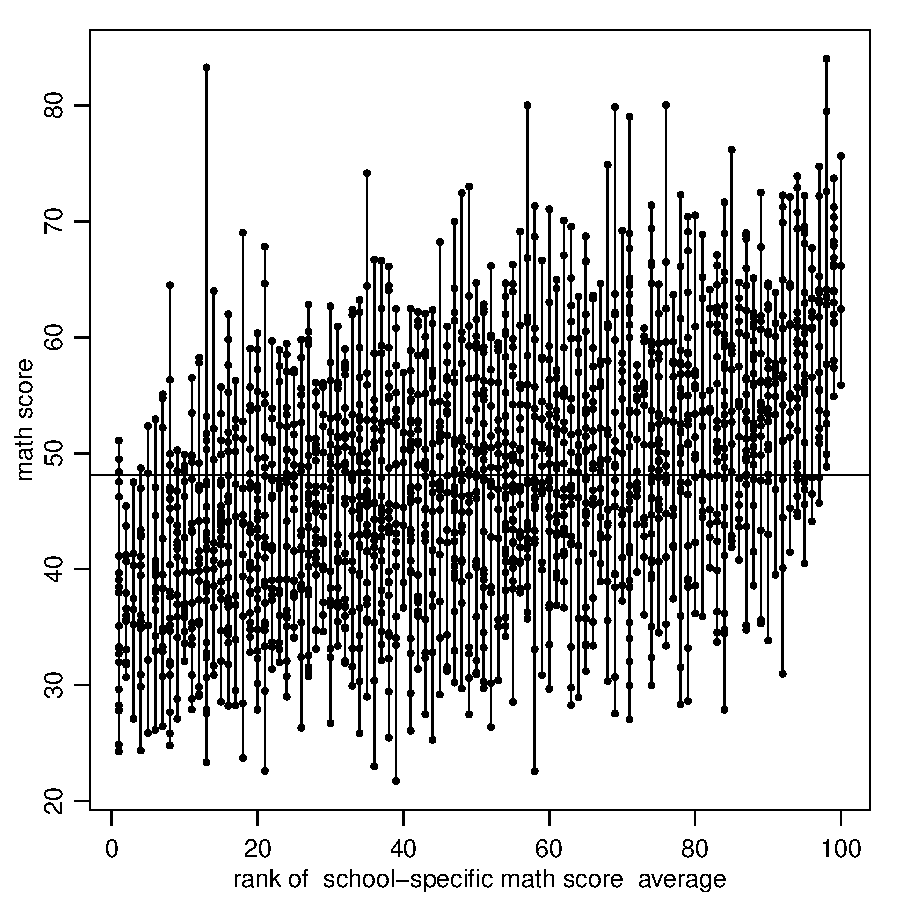
\includegraphics{Thesis_v4-009}



% <<fig=TRUE,echo=FALSE>>=
% #Histogram of school mean scores, and relationship between sample mean and sample size
%
% #pdf("fig8_5.pdf",family="Times",height=3.5,width=7)
% par(mfrow=c(1,2),mar=c(3,3,1,1),mgp=c(1.75,.75,0))
% hist(ybar,main="",xlab="sample mean")
% plot(n,ybar,xlab="sample size",ylab="sample mean")
% #dev.off()

% Note:  to comment out the above chunk, I had to leave the @ uncommented.  Otherwise all that follows gets treated like it's within the chunk starting with the top line here, even though that line is commented.  I don't know why this is the case.

\noindent For prediction, we'll use the following prior values (Hoff p. 137):

      \begin{flalign*}
        \sigma^2_0&:  100 \text{ (within-school variance)}\\
        \nu_0&:  1 \text{ (prior sample size)}\\
        \tau^2_0&:  100 \text{ (between-school variance)}\\
        \eta_0&:  1 \text{ (prior sample size)}\\
        \mu_0&:  50 \text{ (prior mean of school means)}\\
        \gamma^2_0&:  25 \text{ (prior variance of school means)}
      \end{flalign*}

\noindent In the example below the observed test score data from three individual schools are compared with their predictions.  The schools chosen were numbers 5, 67, and 92 from the study, which had the minimum average math score, maximum average math score, and closest to the overall average math score, respectively.


\begin{center}
  \begin{tabular}{|c|c|c|}
    \hline
    & school & average \\
    \hline
    min average & 5 & 36.58 \\
    \hline
    max average & 67 & 65.02 \\
    \hline
    grand mean & -- & 48.13 \\
    \hline
    closest to overall & 92 & 48.18\\
    \hline
  \end{tabular}
\end{center}

\noindent The plot below shows the density curves of the observed math scores for these three schools and the predictions of future math scores.  The observed data is shown using solid lines, and the predictive densities are displayed with dashed lines.  The predictions are ``pulled" toward the overall mean, which is indicated on the plot with the dotted gray vertical line.

\textcolor{red}{As before, what is being predicted?}\\
\textcolor{blue}{See expansion of first sentence in above paragraph.  Does that suffice?}

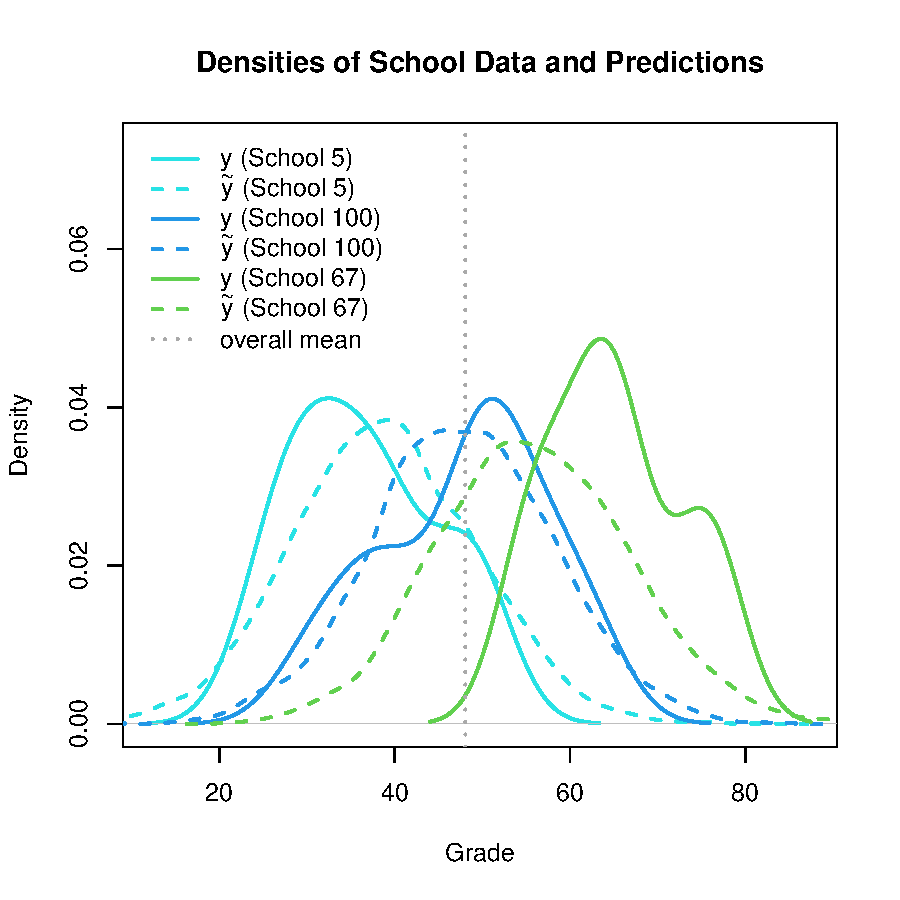
\includegraphics{Thesis_v4-011}


      % \paragraph{Ranking Treatments}

\clearpage


\section{Normal Regression}% with Zellner's $g$-prior}

% \textcolor{red}{intro here}\\
% \textcolor{red}{stipulate variable naming convention here (x is the observed data now).  Modify previous intro to indicate variable convention was for the exponential family set of models}

\noindent Starting with observations $Y_1,...,Y_N$ and explanatory variables $\mathbf{x}_1,...,\mathbf{x}_n$, with $\mathbf{x}_i = \left\{ x_{i,1}, x_{i,2}, ..., x_{i,p} \right\}$ where $Y_i = \boldsymbol\beta^T \mathbf{x}_i + \epsilon_i$ and $\epsilon_1,...,\epsilon_n\overset{\text{i.i.d.}}{\sim} \text{Normal}\left(0,\sigma^2\right)$, we have joint probability density

\begin{flalign}
    p\left(y_1,...y_n|\mathbf{x}_1,...,\mathbf{x}_n,\boldsymbol\beta,\sigma^2\right) &= \prod_{i=1}^n p\left(y_i|\mathbf{x}_i,\boldsymbol\beta,\sigma^2\right) \nonumber\\
    &= \left(2\pi\sigma^2\right)^{-n/2}\text{exp}\left\{-\frac{1}{2\sigma^2}\sum_{i=1}^n\left(y_i - \boldsymbol\beta^T\mathbf{x}_i\right)^2\right\}. \label{regressionJointNorm}
\end{flalign}

\noindent If we let $\mathbf{y}=(y_1,...,y_n)^T$ and let $\mathbf{X}$ be the $n \times p$ matrix whose $i$th row is $\mathbf{x}_i$, then we can express this joint probability in terms of the Multivariate Normal distribution.  The Normal regression model is

$$\{\mathbf{y}|\mathbf{X},\boldsymbol\beta,\sigma^2\} \sim \text{Multivariate Normal}\left(\mathbf{X}\boldsymbol\beta,\sigma^2\mathbf{I}\right),$$

\noindent where $\mathbf{I}$ is the $p \times p$ identity matrix and

\begin{equation*}
    \mathbf{X}\boldsymbol\beta =
    \begin{pmatrix}
        \mathbf{x}_1 \\
        \mathbf{x}_2 \\
        \vdots  \\
        \mathbf{x}_n
    \end{pmatrix}
    \begin{pmatrix}
        \beta_1 \\
        \beta_2 \\
        \vdots \\
        \beta_p
    \end{pmatrix}
    =
    \begin{pmatrix}
        \beta_1 x_{1,1} + \cdots + \beta_p x_{1,p} \\
        \vdots \\
        \beta_1 x_{n,1} + \cdots + \beta_p x_{n,p} \\
    \end{pmatrix}
    =
    \begin{pmatrix}
        E\left[Y_1|\mathbf{\boldsymbol\beta},\mathbf{x}_1\right] \\
        \vdots \\
        E\left[Y_n|\mathbf{\boldsymbol\beta},\mathbf{x}_n\right] \\
    \end{pmatrix}
\end{equation*}

\noindent The density (\ref{regressionJointNorm}) depends on $\boldsymbol\beta$ through the residuals $\left(y_i - \boldsymbol\beta^T\mathbf{x}_i\right)$.  We compute the ordinary least squares estimates

$$\hat{\boldsymbol\beta}_{ols} = \left(\mathbf{X}^T\mathbf{X}\right)^{-1}\mathbf{X}^T\mathbf{y}$$

\noindent and

$$\hat{\sigma}^2_{ols} = \frac{SSR\left(\hat{\boldsymbol\beta}_{ols}\right)}{(n-p)} = \frac{\sum\left(y_i - \hat{\boldsymbol\beta}_{ols}^T x_i\right)^2}{(n-p)}.$$


\noindent Here

\begin{flalign*}
  SSR(\beta) &= \sum_{i=1}^n(y_i-\beta^T x_i)^2\\
              &= \sum_{i=1}^n(\mathbf{y-X}\beta)^T(\mathbf{y-X}\beta)\\
              &= \mathbf{y}^T\mathbf{y}-2\beta^T\mathbf{X}^T\mathbf{y} + \beta^T\mathbf{X}^T\mathbf{X}\beta
\end{flalign*}

\noindent is the sum of squared residuals, which is minimized by $\hat\beta_{ols} = (\mathbf{X^T X})^{-1}X^T y$.\\


\subsection{Least Squares Estimation Example (Hoff p. 149ff.)}

\textcolor{red}{Your example 4.1 is much better described than the other examples. You
should try to bring the others up to this standard.}

\noindent Here we reproduce the example provided by Hoff, which will be used to illustrate Bayesian prediction for a regression model.\\

\noindent\textit{Example:  Oxygen uptake (from Kuehl (2000), Hoff p. 149ff)}

\noindent Twelve healthy men who did not exercise regularly were recruited to take part in a study of the effects of two different exercise regimens on oxygen uptake.  Six of the twelve men were randomly assigned to a 12-week flat-terrain running program, and the remaining six were assigned to a 12-week step aerobics program.  The maximum oxygen uptake of each subject was measured (in liters per minute) while running on an inclined treadmill, both before and after the 12-week program.  Of interest is how a subject's change in maximal oxygen uptake may depend on which program they were assigned to.  However, other factors, such as age, are expected to affect the change in maximal uptake as well.  The results are shown here:

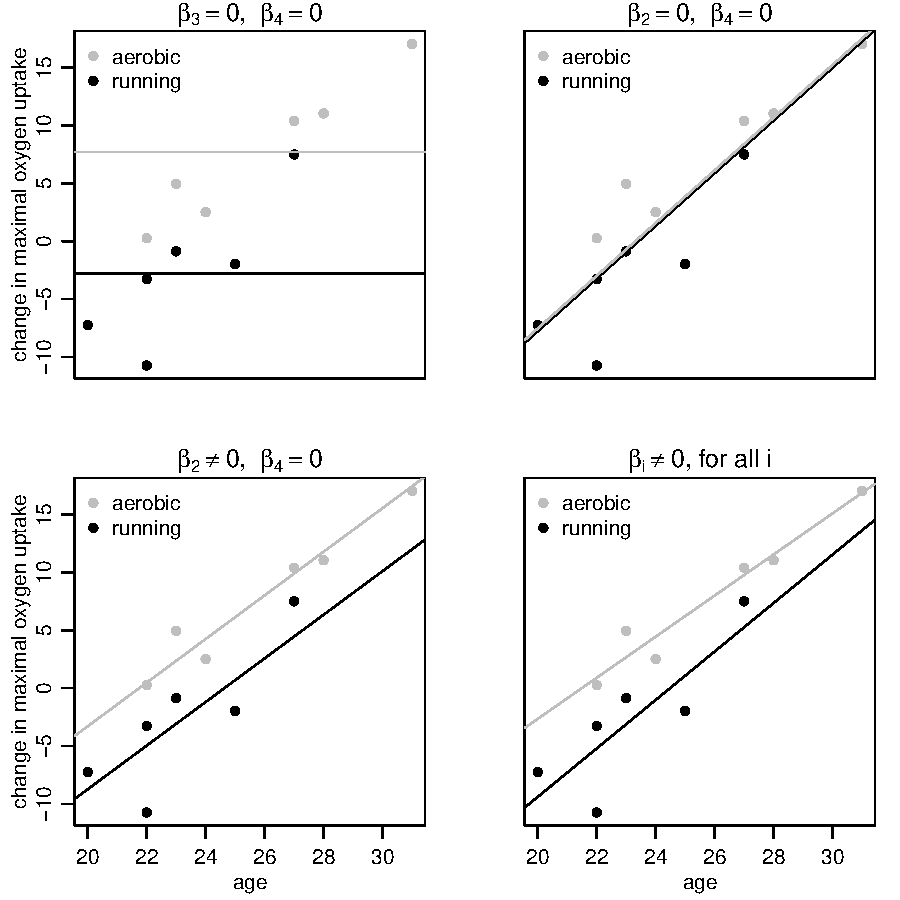
\includegraphics{Thesis_v4-012}

\noindent Hoff's regression model:

    \begin{align}
        Y_i &= \beta_1x_{i,1} + \beta_2x_{i,2} + \beta_3x_{i,3} + \beta_4x_{i,4} + \epsilon_i, \text{ where} \label{example_regression_model}\\
        x_{i,1} &= 1 \text{ for each subject } i \nonumber \\
        x_{i,2} &= 0 \text{ if subject } i \text{ is on the running program, } 1 \text{ if on aerobic} \nonumber \\
        x_{i,3} &= \text{ age of subject } i \nonumber \\
        x_{i,4} &= x_{i,2} \times x_{i,3} \nonumber
    \end{align}

% \textcolor{red}{Here Hoff has this:}
%
% \noindent Under this model the conditional expectations of $Y$ for the two different levels of $x_{i,1}$ are
%
% \begin{flalign*}
%     E[Y|\mathbf{x}] &= \beta_1 + \beta_3 \times (age) \text{ if } x_1 = 0, \text{ and}\\
%     E[Y|\mathbf{x}] &= \left(\beta_1 + \beta_2\right) + \left(\beta_3 + \beta_4\right) \times (age) \text{ if } x_1 = 1
% \end{flalign*}

% \textcolor{red}{But I think he means this:}

\noindent Under this model the conditional expectations of $Y$ for the two different levels of $x_{i,2}$ are

\begin{flalign*}
    E[Y|\mathbf{x}] &= \beta_1 + \beta_3 \times (age) \text{ if } x_{i,2} = 0 \text{ (running program), and}\\
    E[Y|\mathbf{x}] &= \left(\beta_1 + \beta_2\right) + \left(\beta_3 + \beta_4\right) \times (age) \text{ if } x_{i,2} = 1 \text{ (aerobic program) }
\end{flalign*}

\noindent In other words, the model assumes that the relationship is linear in age for both exercise groups, with the difference in intercepts given by $\beta_2$ and the difference in slopes given by $\beta_4$.  If we assumed that $\beta_2 = \beta_4 = 0$, then we would have identical lines for both groups.  If we assumed $\beta_2 \ne 0$ and $\beta_4 =  0$ then we would have a different line for each group but they would be parallel.  Allowing all coefficients to be non-zero gives us two unrelated lines.  Some different possibilities are depicted graphically below:\\\\

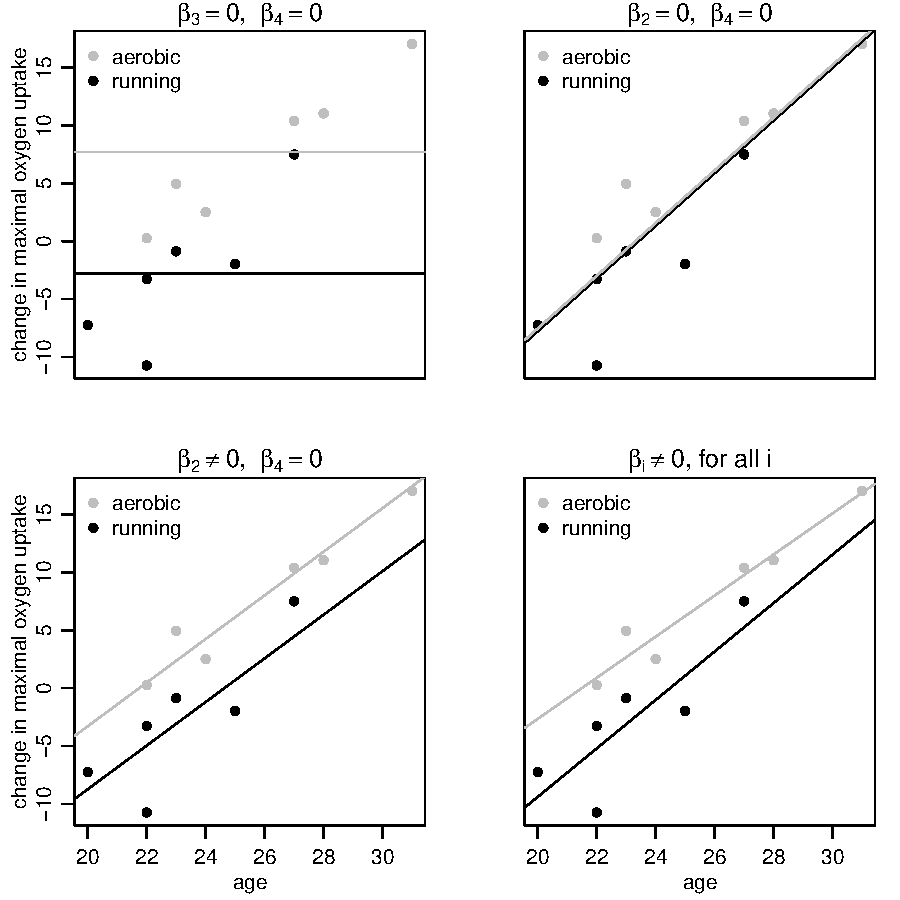
\includegraphics{Thesis_v4-013}

\noindent Let's find the least squares regression estimates for the model (\ref{example_regression_model}), and use the results to evaluate the differences between the two exercise groups.  The ages of the 12 subjects, along with their observed changes in maximal oxygen uptake, are

\begin{flalign*}
    \mathbf{x}_3 &= (23,22,22,25,27,20,31,23,27,28,22,24)\\
    \mathbf{y}   &= (-0.87,-10.74,-3.27,-1.97,7.50,-7.25,17.05,4.96,10.40,11.05,0.26,2.51),
\end{flalign*}

\noindent with the first six elements of each vector corresponding to the subjects in the running group and the latter six corresponding to subjects in the aerobics group.  After constructing the $12 \times 4$ matrix $\mathbf{X} = (\mathbf{x}_1\, \mathbf{x}_2\, \mathbf{x}_3\, \mathbf{x}_4)$, the matrices $\mathbf{X}^T\mathbf{X}$ and $\mathbf{X}^T\mathbf{y}$ can be computed, from which we get $\boldsymbol\beta_{ols} = (-51.29,13.11,2.09,-0.32)^T$:\\

\noindent This means that the estimated linear relationship between uptake and age has an intercept and slope of -51.29 and 2.09 for the running group, and -51.29 + 13.11 = -38.18 and 2.09 - 0.32 = 1.77 for the aerobics group.  These two lines are plotted in the fourth panel of Figure XX.  We obtain unbiased estimate $\sigma^2 = SSR(\hat{\boldsymbol\beta}_{ols})/(n-p) = 8.54$, and use this to compute the standard error of the components of $\hat{\boldsymbol\beta}_{ols}$, which are 12.25, 15.76, 0.53, and 0.65, respectively.  Comparing the values of $\hat{\boldsymbol\beta}_{ols}$ to their standard errors suggests that the evidence for differences between the two exercise regimens is not very strong.

% \hrulefill \\
%
% \textcolor{red}{``Comparing the values of $\hat{\boldsymbol\beta}_{ols}$ to their standard errors:"}\\
% Difference in Intercept:\\
% $$H_0:  Intercept_{running} - Intercept_{aerobic} = 0; H_A:  Intercept_{running} - Intercept_{aerobic} \ne 0$$
% $$H_0:  \beta_1 - (\beta_1 + \beta_2) = -\beta_2 = 0 \text{ (that is } \beta_2 = 0); H_A:  \beta_2 \ne 0$$
% $$T = \frac{\beta_2 - 0}{SE_{beta_2}} = \frac{13.11}{15.76} = 0.49$$
% $$\longrightarrow p = 0.79\longrightarrow \text{ fail to reject } H_0 \text{ and conclude no significant difference in intercept}$$
%
% Difference in Slope:\\
% $$H_0:  Slope_{running} - Slope_{aerobic} = 0; H_A:  Slope_{running} - Slope_{aerobic} \ne 0$$
% $$H_0:  \beta_3 - (\beta_3 + \beta_4) = 0 \text{ (that is } \beta_4 = 0); H_A:  \beta_4 \ne 0$$
% $$T = \frac{\beta_4 - 0}{SE_{beta_4}} = \frac{-0.32}{0.65} = 0.83$$
% $$\longrightarrow p = 0.68\longrightarrow \text{ fail to reject } H_0 \text{ and conclude no significant difference in slope}$$
%
%
% \hrulefill \\




\clearpage

  \subsection{Bayesian Estimation for a Regression Model (Hoff p. 154ff)}

  \subsubsection{Derivation}

    \paragraph{A semiconjugate prior distribution}\label{normRegSemiconjugatePrior}
    Hoff proposes a semiconjugate prior distribution for $\boldsymbol\beta$ and $\sigma^2$ to be used when there is information available about the parameters.  The sampling density of the data is

\textcolor{red}{define SSR(beta)
I think you should write out the full conditional distributions for the
different parts of the updating scheme, or at least the expressions for V and m.
Similar to what you did in Chapter 3.}  \textcolor{blue}{See below def of SSR and Gibbs sampler steps with V and m written out.  Better?}

    $$p(\mathbf{y}|\mathbf{X},\boldsymbol\beta,\sigma^2) \propto \text{exp}\{-\frac{1}{2\sigma^2}\text{SSR}(\boldsymbol\beta)\} = \text{exp}\{-\frac{1}{2\sigma^2}[\mathbf{y}^T\mathbf{y} - 2\boldsymbol\beta^T\mathbf{X}^T\mathbf{y}+\boldsymbol\beta^T\mathbf{X}^T\mathbf{X}\boldsymbol\beta]\},$$

\noindent and for priors we choose $\boldsymbol\beta \sim \text{Multivariate Normal}(\boldsymbol\beta_0,\Sigma_0)$ and $1/\sigma^2 = \gamma\sim \text{Gamma}(\nu_0/2,\nu_0\sigma^2_0/2)$.  \\
%
% \noindent Here
%
% \begin{flalign*}
%   SSR(\beta) &= \sum_{i=1}^n(y_i-\beta^T x_i)^2\\
%               &= \sum_{i=1}^n(\mathbf{y-X}\beta)^T(\mathbf{y-X}\beta)\\
%               &= \mathbf{y}^T\mathbf{y}-2\beta^T\mathbf{X}^T\mathbf{y} + \beta^T\mathbf{X}^T\mathbf{X}\beta
% \end{flalign*}
%
% \noindent is the sum of squared residuals, which is minimized by the ordinary least squares estimate $\beta_{ols} = (\mathbf{X^T X})^{-1}X^T y$.\\

\noindent Thus we have

    \begin{flalign*}
        p&(\boldsymbol\beta|\mathbf{y,X},\sigma^2)\\
        &\propto p(\mathbf{y}|\mathbf{X},\boldsymbol\beta, \sigma^2) \times p(\boldsymbol\beta)\\
        &\propto \text{exp}\{-\frac{1}{2}(-2\boldsymbol\beta^T\mathbf{X}^T\mathbf{y}/\sigma^2 + \boldsymbol\beta^T\mathbf{X}^T\mathbf{X}\boldsymbol\beta/\sigma^2) - \frac{1}{2}(-2\boldsymbol\beta^T\Sigma_0^{-1}\boldsymbol\beta_0 + \boldsymbol\beta^T\Sigma_0^{-1}\boldsymbol\beta)\}\\
        &=\text{exp}\{\boldsymbol\beta^T(\Sigma_0^{-1}\boldsymbol\beta_0 + \mathbf{X}^T\mathbf{y}/\sigma^2) - \frac{1}{2}\boldsymbol\beta^T(\Sigma_0^{-1} + \mathbf{X}^T\mathbf{X}/\sigma^2)\boldsymbol\beta\}
    \end{flalign*}

\noindent and

\begin{flalign*}
    p(\gamma|\mathbf{y,X},\boldsymbol\beta) &\propto p(\gamma)p(\mathbf{y}|\mathbf{X},\boldsymbol\beta,\gamma)\\
        &\propto \left[\gamma^{\nu_0/2-1}\text{exp}(-\gamma \times \nu_0\sigma^2_0/2)\right] \times
                 \left[\gamma^{n/2}\text{exp}(-\gamma \times \text{SSR}(\boldsymbol\beta)/2)\right]\\
        &= \gamma^{(\nu_0+n)/2-1} \text{exp}(-\gamma[\nu_0\sigma^2_0 + \text{SSR}(\boldsymbol\beta)]/2),
\end{flalign*}

\noindent which we recognize as a gamma density, so that

$$\{\sigma^2|\mathbf{y,X},\boldsymbol\beta\} \sim \text{Inverse Gamma}([\nu_0 + n]/2,[\nu_0\sigma^2_0 + \text{SSR}(\boldsymbol\beta)]/2).$$

\vspace{5mm}

\noindent Constructing a Gibbs sampler to approximate the joint posterior distribution $p(\boldsymbol\beta,\sigma^2|\mathbf{y,X})$ is then straightforward:  given current values $\{\boldsymbol\beta^{(s)},\sigma^{2(s)}\}$, new values can be generated by

\begin{enumerate}
    \item updating $\boldsymbol\beta$:
    \begin{enumerate}
        \item compute $\mathbf{V} = \text{Var}[\boldsymbol\beta|\mathbf{y,X},\sigma^{2(s)}] = \left(\Sigma_0^{-1} + \mathbf{X}^T\mathbf{X}/\sigma^{2(s)}\right)^{-1}$ and \\$\mathbf{m} = \text{E}[\boldsymbol\beta|\mathbf{y,X},\sigma^{2(s)}] = \left(\Sigma_0^{-1} + \mathbf{X}^T\mathbf{X}/\sigma^{2(s)}\right)^{-1}\left(\Sigma_0^{-1}\beta_0 + \mathbf{X}^T\mathbf{y}/\sigma^{2(s)}\right)$
        \item sample $\boldsymbol\beta^{(s+1)} \sim \text{Multivariate Normal}(\mathbf{m,V})$
    \end{enumerate}
    \item updating $\sigma^2$:
    \begin{enumerate}
        \item compute SSR$(\boldsymbol\beta^{(s+1)})$
        \item sample $\sigma^{2(s+1)} \sim \text{Inverse Gamma}([\nu_0 + n]/2,[\nu_0\sigma_0^2 + \text{SSR}(\boldsymbol\beta^{(s+1)})]/2)$.
    \end{enumerate}
\end{enumerate}

To create a sample from the predictive distribution of responses:  for each $s\in\{1,...,S\}$, draw $\epsilon^{(s)} \sim \text{Normal}(0,\sigma^{2(s)})$.  Then compute

$$y^{(s)} = \boldsymbol\beta^{(s)T}\mathbf{X} + \epsilon.$$

    \paragraph{Default and weakly informative prior distributions}

    In situations where prior information is unavailable or difficult to quantify, an alternative ``default" class of prior distributions is given. Here we will employ Zellner's ``$g$-prior" (Zellner, 1986).  We choose $\boldsymbol\beta_0 = \mathbf{0}$ and $\Sigma_0 = k(\mathbf{X}^T\mathbf{X})^{-1}, k = g\sigma^2, g > 0$, which satisfies a desired condition that the regression parameter estimation be invariant to changes in the scale of the regressors.  Note that this prior conditions on the observed $\mathbf{X}$ matrix.With this, equations \ref{regression_semiconj_var} and \ref{regression_semiconj_expec} reduce to

\begin{flalign}
    \text{Var}[\boldsymbol\beta|\mathbf{y,X},\sigma^2] &= [\mathbf{X^TX}/(g\sigma^2) + \mathbf{X^TX}/\sigma^2]^{-1} = \frac{g}{g+1}\sigma^2(\mathbf{X^TX})^{-1} \label{regression_noninf_var}\\
    \text{E}[\boldsymbol\beta|\mathbf{y,X},\sigma^2] &= [\mathbf{X^TX}/(g\sigma^2) + \mathbf{X^TX}/\sigma^2]^{-1}\mathbf{X^Ty}/\sigma^2 = \frac{g}{g+1}\sigma^2(\mathbf{X^TX})^{-1}\mathbf{X^Ty}.\label{regression_noninf_expec}
\end{flalign}

\noindent Letting

$$\mathbf{V} = \frac{g}{g+1}\sigma^2(\mathbf{X^TX})^{-1} \text{ and } \mathbf{m} = \frac{g}{g+1}\sigma^2(\mathbf{X^TX})^{-1}\mathbf{X^Ty}$$

\noindent we arrive at posteriors

\begin{flalign}
    \{\sigma^2|\mathbf{y,X}\} &\sim \text{Inverse Gamma}([\nu_0 + n]/2,[\nu_0\sigma^2_0 + \text{SSR}_g]/2) \label{regression_noninf_sig2_post}\\
    \{\boldsymbol\beta|\mathbf{y,X},\sigma^2\} &\sim \text{Multivariate Normal}\left(\frac{g}{g+1}\hat{\boldsymbol\beta}_{ols},\frac{g}{g+1}\sigma^2[\mathbf{X^TX}]^{-1}\right).\label{regression_noninf_beta_post}
\end{flalign}

\noindent Here $\text{SSR}_g = \mathbf{y^Ty - m^TV^{-1}m = y^T(I - }\frac{g}{g+1}\mathbf{X(X^TX)^{-1}X^T)y}$.\\

Simple monte carlo approximation can be used to sample from the joint posterior density $p(\sigma^2,\boldsymbol\beta|\mathbf{y,X})$ as follows.  Here $g$ is typically set to the size of the data sample. Then:

\begin{enumerate}
    \item sample $\sigma^2 \sim \text{Inverse Gamma}([\nu_0 + n]/2,[\nu_0\sigma^2_0 + \text{SSR}_g]/2)$
    \item sample $\boldsymbol\beta \sim \text{Multivariate Normal}\left(\frac{g}{g+1}\hat{\boldsymbol\beta}_{ols},\frac{g}{g+1}\sigma^2[\mathbf{X^TX}]^{-1}\right)$.
\end{enumerate}

\noindent To create a sample from the predictive distribution of responses, draw $\epsilon \sim \text{Normal}(0,\sigma^2)$.  Then for each triplet $(\beta,\sigma^2,\epsilon)$ we have

$$y = \boldsymbol\beta^T\mathbf{X} + \epsilon.$$

  \subsubsection{R Implementation (Normal Regression)}

The R function \texttt{rpredNormReg(S,Xpred,X,y,beta0,Sigma0,nu0,s20,gprior)}

\noindent approximates the joint posterior density $p(\sigma^2,\boldsymbol\beta|\mathbf{y,X})$ using one of the two methods described above, generates $S$ triplets $(\boldsymbol\beta^{(s)}, \sigma^{2(s)},\epsilon^{(s)} \sim \text{Normal}(0,\sigma^{2(s)})$ , and returns $S$ predictions $y = X_{pred}\boldsymbol\beta^{(s)} + \epsilon^{(s)}$.  Calls to this functions appear as follows:


\begin{center}
  \texttt{rpredNormReg(S,Xpred,X,y,beta0,Sigma0,nu0,s20,gprior)}\\
\end{center}

\noindent where

\begin{flalign*}
  \texttt{S} &= S \text{, the number of MCMC realizations (the desired random sample size)}\\
  \texttt{Xpred} &= \text{ the vector or matrix of vectors of explanatory variables upon which to base}\\ &\text{prediction }\\
  \texttt{X} &= \mathbf{X} \text{, the design matrix associated with the observed data}\\
  \texttt{y} &= \mathbf{y} \text{, the observed response vector}\\
  \texttt{beta0} &= \beta_0 \text{, location vector for the Multivariate Normal prior distribution of } \mathbf{\beta}\\
  \texttt{Sigma0} &= \Sigma_0 \text{, covariance matrix for the Multivariate Normal prior distribution of } \mathbf{\beta}\\
  \texttt{nu0,s20} &= \nu_0,\sigma^2_0 \text{, prior parameters for the Inverse-Gamma prior distribution of }\sigma^2\\
  \texttt{gprior} &= \text{ a flag controlling the decision to use Zellner's location-invariant g-prior}
\end{flalign*}

\noindent Note:  the function defaults to \texttt{gprior=TRUE}, in which case input values for \texttt{beta0, Sigma0, nu0}, and \texttt{s20} are ignored.  If the user wants to employ Hoff's semi-conjugate prior as defined in section \ref{normRegSemiconjugatePrior} above, all input variables must be specified, with \texttt{gprior = FALSE}.




  \subsubsection{Example}

In the example below (Hoff data and code found \href{https://pdhoff.github.io/book/}{here}) to employ Hoff's semi-conjugate prior we use



\begin{flalign*}
  \boldsymbol\beta_0 &= \hat{\boldsymbol\beta}_{ols} = (-51.29, -51.29, -51.29, -51.29)  \text{ (ordinary least squares estimator of } \boldsymbol\beta \text{)}\\
  \Sigma_0 &= (X^TX)^{-1}\sigma^2n =
    \begin{pmatrix}
      1801.4 & -1801.4 & -77.02 & 77.02 \\
      -1801.4 & 2981.28 & 77.02 & -122.03 \\
      -77.02 & 77.02 & 3.32 & -3.32 \\
      77.02 & -122.03 & -3.32 & 5.07
    \end{pmatrix}
    \text{ (sampling variance of } \hat{\boldsymbol\beta}_{ols}\text{)}\\%\text{WHY TIMES n????}\\
  \nu_0 &= 1 \text{ (prior sample size)}\\
  \sigma^2_0 &= \frac{\sum e_i}{n-1} = 6.21 \text{ (variance of the residuals)}\\
  S &= 5000 \text{ (sample size for predictive distribution random draw)}
\end{flalign*}


\noindent Inspection of the plot below shows the predicted distributions using Zellner's g-prior shrink toward 0, and have greater variance than those predicted using Hoff's semi-conjugate prior.

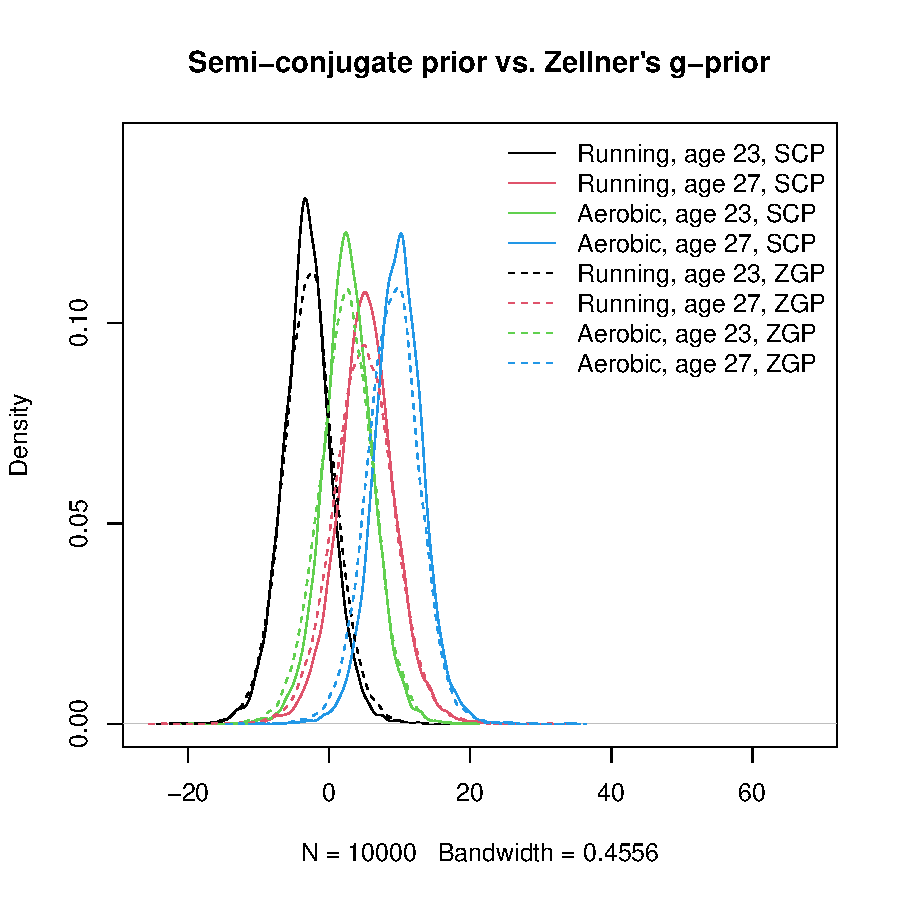
\includegraphics{Thesis_v4-016}


\clearpage

\section{Conclusion}

\section{Appendix}

\section{References}

\end{document}
